\documentclass{article}
\usepackage[final]{neurips_2025}  % NEURIPS style (neurips_2025.sty is in paper_draft/)
\makeatletter\providecommand{\@trackname}{\@neuripsordinal\ Conference on Neural Information Processing Systems (NeurIPS \@neuripsyear).}\makeatother
\usepackage[hidelinks]{hyperref}  % REQUIRED: clickable links
\usepackage{booktabs}  % REQUIRED: professional tables
\usepackage{graphicx}
\usepackage{amsmath,amssymb}
\usepackage[utf8]{inputenc}
\usepackage[T1]{fontenc}
\usepackage{enumitem}
\usepackage{multirow}
\usepackage{algorithm}
\usepackage[noend]{algpseudocode}

% Import command files
%%%%% MATH NOTATION MACROS %%%%%
% Standard math notation for academic papers
% Import with: %%%%% MATH NOTATION MACROS %%%%%
% Standard math notation for academic papers
% Import with: %%%%% MATH NOTATION MACROS %%%%%
% Standard math notation for academic papers
% Import with: \input{commands/math}

\usepackage{amsmath,amsfonts,bm}

%%%%%%%%%%%%%%%%%%%%%%%%%%%%%%%%%%%%%%%%%%%%%%%%%%%%%%%%%%%%%%%%%
% FIGURE AND SECTION REFERENCES
%%%%%%%%%%%%%%%%%%%%%%%%%%%%%%%%%%%%%%%%%%%%%%%%%%%%%%%%%%%%%%%%%

% Mark sections of captions for referring to divisions of figures
\newcommand{\figleft}{{\em (Left)}}
\newcommand{\figcenter}{{\em (Center)}}
\newcommand{\figright}{{\em (Right)}}
\newcommand{\figtop}{{\em (Top)}}
\newcommand{\figbottom}{{\em (Bottom)}}
\newcommand{\captiona}{{\em (a)}}
\newcommand{\captionb}{{\em (b)}}
\newcommand{\captionc}{{\em (c)}}
\newcommand{\captiond}{{\em (d)}}

% Figure references
\def\figref#1{figure~\ref{#1}}
\def\Figref#1{Figure~\ref{#1}}
\def\twofigref#1#2{figures \ref{#1} and \ref{#2}}
\def\quadfigref#1#2#3#4{figures \ref{#1}, \ref{#2}, \ref{#3} and \ref{#4}}

% Section references
\def\secref#1{section~\ref{#1}}
\def\Secref#1{Section~\ref{#1}}
\def\twosecrefs#1#2{sections \ref{#1} and \ref{#2}}
\def\secrefs#1#2#3{sections \ref{#1}, \ref{#2} and \ref{#3}}

% Equation references
\def\eqref#1{equation~\ref{#1}}
\def\Eqref#1{Equation~\ref{#1}}
\def\plaineqref#1{\ref{#1}}

% Algorithm references
\def\algref#1{algorithm~\ref{#1}}
\def\Algref#1{Algorithm~\ref{#1}}
\def\twoalgref#1#2{algorithms \ref{#1} and \ref{#2}}
\def\Twoalgref#1#2{Algorithms \ref{#1} and \ref{#2}}

% Table references
\def\tabref#1{table~\ref{#1}}
\def\Tabref#1{Table~\ref{#1}}

% Chapter references
\def\chapref#1{chapter~\ref{#1}}
\def\Chapref#1{Chapter~\ref{#1}}

%%%%%%%%%%%%%%%%%%%%%%%%%%%%%%%%%%%%%%%%%%%%%%%%%%%%%%%%%%%%%%%%%
% BASIC MATH DEFINITIONS
%%%%%%%%%%%%%%%%%%%%%%%%%%%%%%%%%%%%%%%%%%%%%%%%%%%%%%%%%%%%%%%%%

\def\ceil#1{\lceil #1 \rceil}
\def\floor#1{\lfloor #1 \rfloor}
\def\1{\bm{1}}
\def\eps{{\epsilon}}

% Common operators
\DeclareMathOperator*{\argmax}{arg\,max}
\DeclareMathOperator*{\argmin}{arg\,min}
\DeclareMathOperator{\sign}{sign}
\DeclareMathOperator{\Tr}{Tr}
\let\ab\allowbreak

%%%%%%%%%%%%%%%%%%%%%%%%%%%%%%%%%%%%%%%%%%%%%%%%%%%%%%%%%%%%%%%%%
% VECTORS (lowercase bold)
%%%%%%%%%%%%%%%%%%%%%%%%%%%%%%%%%%%%%%%%%%%%%%%%%%%%%%%%%%%%%%%%%

\def\vzero{{\bm{0}}}
\def\vone{{\bm{1}}}
\def\vmu{{\bm{\mu}}}
\def\vtheta{{\bm{\theta}}}
\def\va{{\bm{a}}}
\def\vb{{\bm{b}}}
\def\vc{{\bm{c}}}
\def\vd{{\bm{d}}}
\def\ve{{\bm{e}}}
\def\vf{{\bm{f}}}
\def\vg{{\bm{g}}}
\def\vh{{\bm{h}}}
\def\vi{{\bm{i}}}
\def\vj{{\bm{j}}}
\def\vk{{\bm{k}}}
\def\vl{{\bm{l}}}
\def\vm{{\bm{m}}}
\def\vn{{\bm{n}}}
\def\vo{{\bm{o}}}
\def\vp{{\bm{p}}}
\def\vq{{\bm{q}}}
\def\vr{{\bm{r}}}
\def\vs{{\bm{s}}}
\def\vt{{\bm{t}}}
\def\vu{{\bm{u}}}
\def\vv{{\bm{v}}}
\def\vw{{\bm{w}}}
\def\vx{{\bm{x}}}
\def\vy{{\bm{y}}}
\def\vz{{\bm{z}}}

%%%%%%%%%%%%%%%%%%%%%%%%%%%%%%%%%%%%%%%%%%%%%%%%%%%%%%%%%%%%%%%%%
% MATRICES (uppercase bold)
%%%%%%%%%%%%%%%%%%%%%%%%%%%%%%%%%%%%%%%%%%%%%%%%%%%%%%%%%%%%%%%%%

\def\mA{{\bm{A}}}
\def\mB{{\bm{B}}}
\def\mC{{\bm{C}}}
\def\mD{{\bm{D}}}
\def\mE{{\bm{E}}}
\def\mF{{\bm{F}}}
\def\mG{{\bm{G}}}
\def\mH{{\bm{H}}}
\def\mI{{\bm{I}}}
\def\mJ{{\bm{J}}}
\def\mK{{\bm{K}}}
\def\mL{{\bm{L}}}
\def\mM{{\bm{M}}}
\def\mN{{\bm{N}}}
\def\mO{{\bm{O}}}
\def\mP{{\bm{P}}}
\def\mQ{{\bm{Q}}}
\def\mR{{\bm{R}}}
\def\mS{{\bm{S}}}
\def\mT{{\bm{T}}}
\def\mU{{\bm{U}}}
\def\mV{{\bm{V}}}
\def\mW{{\bm{W}}}
\def\mX{{\bm{X}}}
\def\mY{{\bm{Y}}}
\def\mZ{{\bm{Z}}}
\def\mBeta{{\bm{\beta}}}
\def\mPhi{{\bm{\Phi}}}
\def\mLambda{{\bm{\Lambda}}}
\def\mSigma{{\bm{\Sigma}}}

%%%%%%%%%%%%%%%%%%%%%%%%%%%%%%%%%%%%%%%%%%%%%%%%%%%%%%%%%%%%%%%%%
% CALLIGRAPHIC (mathcal)
%%%%%%%%%%%%%%%%%%%%%%%%%%%%%%%%%%%%%%%%%%%%%%%%%%%%%%%%%%%%%%%%%

\def\gA{{\mathcal{A}}}
\def\gB{{\mathcal{B}}}
\def\gC{{\mathcal{C}}}
\def\gD{{\mathcal{D}}}
\def\gE{{\mathcal{E}}}
\def\gF{{\mathcal{F}}}
\def\gG{{\mathcal{G}}}
\def\gH{{\mathcal{H}}}
\def\gI{{\mathcal{I}}}
\def\gJ{{\mathcal{J}}}
\def\gK{{\mathcal{K}}}
\def\gL{{\mathcal{L}}}
\def\gM{{\mathcal{M}}}
\def\gN{{\mathcal{N}}}
\def\gO{{\mathcal{O}}}
\def\gP{{\mathcal{P}}}
\def\gQ{{\mathcal{Q}}}
\def\gR{{\mathcal{R}}}
\def\gS{{\mathcal{S}}}
\def\gT{{\mathcal{T}}}
\def\gU{{\mathcal{U}}}
\def\gV{{\mathcal{V}}}
\def\gW{{\mathcal{W}}}
\def\gX{{\mathcal{X}}}
\def\gY{{\mathcal{Y}}}
\def\gZ{{\mathcal{Z}}}

%%%%%%%%%%%%%%%%%%%%%%%%%%%%%%%%%%%%%%%%%%%%%%%%%%%%%%%%%%%%%%%%%
% SETS (blackboard bold)
%%%%%%%%%%%%%%%%%%%%%%%%%%%%%%%%%%%%%%%%%%%%%%%%%%%%%%%%%%%%%%%%%

\def\sA{{\mathbb{A}}}
\def\sB{{\mathbb{B}}}
\def\sC{{\mathbb{C}}}
\def\sD{{\mathbb{D}}}
\def\sF{{\mathbb{F}}}
\def\sG{{\mathbb{G}}}
\def\sH{{\mathbb{H}}}
\def\sI{{\mathbb{I}}}
\def\sJ{{\mathbb{J}}}
\def\sK{{\mathbb{K}}}
\def\sL{{\mathbb{L}}}
\def\sM{{\mathbb{M}}}
\def\sN{{\mathbb{N}}}
\def\sO{{\mathbb{O}}}
\def\sP{{\mathbb{P}}}
\def\sQ{{\mathbb{Q}}}
\def\sR{{\mathbb{R}}}
\def\sS{{\mathbb{S}}}
\def\sT{{\mathbb{T}}}
\def\sU{{\mathbb{U}}}
\def\sV{{\mathbb{V}}}
\def\sW{{\mathbb{W}}}
\def\sX{{\mathbb{X}}}
\def\sY{{\mathbb{Y}}}
\def\sZ{{\mathbb{Z}}}

%%%%%%%%%%%%%%%%%%%%%%%%%%%%%%%%%%%%%%%%%%%%%%%%%%%%%%%%%%%%%%%%%
% COMMON MATH SHORTCUTS
%%%%%%%%%%%%%%%%%%%%%%%%%%%%%%%%%%%%%%%%%%%%%%%%%%%%%%%%%%%%%%%%%

% Expectation and variance
\newcommand{\E}{\mathbb{E}}
\newcommand{\Var}{\mathrm{Var}}
\newcommand{\Cov}{\mathrm{Cov}}
\newcommand{\R}{\mathbb{R}}

% Datasets
\newcommand{\train}{\mathcal{D}}
\newcommand{\valid}{\mathcal{D_{\mathrm{valid}}}}
\newcommand{\test}{\mathcal{D_{\mathrm{test}}}}

% Distributions
\newcommand{\laplace}{\mathrm{Laplace}}
\newcommand{\Uniform}{\mathrm{Unif}}
\newcommand{\Normal}{\mathrm{Normal}}
\newcommand{\Categorical}{\mathrm{Categorical}}

% Common functions
\newcommand{\softmax}{\mathrm{softmax}}
\newcommand{\sigmoid}{\sigma}
\newcommand{\KL}{D_{\mathrm{KL}}}

% Norms
\newcommand{\normlzero}{L^0}
\newcommand{\normlone}{L^1}
\newcommand{\normltwo}{L^2}
\newcommand{\normlp}{L^p}
\newcommand{\normmax}{L^\infty}

%%%%%%%%%%%%%%%%%%%%%%%%%%%%%%%%%%%%%%%%%%%%%%%%%%%%%%%%%%%%%%%%%
% DEFINITIONS AND HIGHLIGHTING
%%%%%%%%%%%%%%%%%%%%%%%%%%%%%%%%%%%%%%%%%%%%%%%%%%%%%%%%%%%%%%%%%

% Highlight a newly defined term
\newcommand{\newterm}[1]{{\bf #1}}
\newcommand{\defn}[1]{\textbf{#1}}
\newcommand{\defeq}{\mathrel{\stackrel{\textnormal{\tiny def}}{=}}}


\usepackage{amsmath,amsfonts,bm}

%%%%%%%%%%%%%%%%%%%%%%%%%%%%%%%%%%%%%%%%%%%%%%%%%%%%%%%%%%%%%%%%%
% FIGURE AND SECTION REFERENCES
%%%%%%%%%%%%%%%%%%%%%%%%%%%%%%%%%%%%%%%%%%%%%%%%%%%%%%%%%%%%%%%%%

% Mark sections of captions for referring to divisions of figures
\newcommand{\figleft}{{\em (Left)}}
\newcommand{\figcenter}{{\em (Center)}}
\newcommand{\figright}{{\em (Right)}}
\newcommand{\figtop}{{\em (Top)}}
\newcommand{\figbottom}{{\em (Bottom)}}
\newcommand{\captiona}{{\em (a)}}
\newcommand{\captionb}{{\em (b)}}
\newcommand{\captionc}{{\em (c)}}
\newcommand{\captiond}{{\em (d)}}

% Figure references
\def\figref#1{figure~\ref{#1}}
\def\Figref#1{Figure~\ref{#1}}
\def\twofigref#1#2{figures \ref{#1} and \ref{#2}}
\def\quadfigref#1#2#3#4{figures \ref{#1}, \ref{#2}, \ref{#3} and \ref{#4}}

% Section references
\def\secref#1{section~\ref{#1}}
\def\Secref#1{Section~\ref{#1}}
\def\twosecrefs#1#2{sections \ref{#1} and \ref{#2}}
\def\secrefs#1#2#3{sections \ref{#1}, \ref{#2} and \ref{#3}}

% Equation references
\def\eqref#1{equation~\ref{#1}}
\def\Eqref#1{Equation~\ref{#1}}
\def\plaineqref#1{\ref{#1}}

% Algorithm references
\def\algref#1{algorithm~\ref{#1}}
\def\Algref#1{Algorithm~\ref{#1}}
\def\twoalgref#1#2{algorithms \ref{#1} and \ref{#2}}
\def\Twoalgref#1#2{Algorithms \ref{#1} and \ref{#2}}

% Table references
\def\tabref#1{table~\ref{#1}}
\def\Tabref#1{Table~\ref{#1}}

% Chapter references
\def\chapref#1{chapter~\ref{#1}}
\def\Chapref#1{Chapter~\ref{#1}}

%%%%%%%%%%%%%%%%%%%%%%%%%%%%%%%%%%%%%%%%%%%%%%%%%%%%%%%%%%%%%%%%%
% BASIC MATH DEFINITIONS
%%%%%%%%%%%%%%%%%%%%%%%%%%%%%%%%%%%%%%%%%%%%%%%%%%%%%%%%%%%%%%%%%

\def\ceil#1{\lceil #1 \rceil}
\def\floor#1{\lfloor #1 \rfloor}
\def\1{\bm{1}}
\def\eps{{\epsilon}}

% Common operators
\DeclareMathOperator*{\argmax}{arg\,max}
\DeclareMathOperator*{\argmin}{arg\,min}
\DeclareMathOperator{\sign}{sign}
\DeclareMathOperator{\Tr}{Tr}
\let\ab\allowbreak

%%%%%%%%%%%%%%%%%%%%%%%%%%%%%%%%%%%%%%%%%%%%%%%%%%%%%%%%%%%%%%%%%
% VECTORS (lowercase bold)
%%%%%%%%%%%%%%%%%%%%%%%%%%%%%%%%%%%%%%%%%%%%%%%%%%%%%%%%%%%%%%%%%

\def\vzero{{\bm{0}}}
\def\vone{{\bm{1}}}
\def\vmu{{\bm{\mu}}}
\def\vtheta{{\bm{\theta}}}
\def\va{{\bm{a}}}
\def\vb{{\bm{b}}}
\def\vc{{\bm{c}}}
\def\vd{{\bm{d}}}
\def\ve{{\bm{e}}}
\def\vf{{\bm{f}}}
\def\vg{{\bm{g}}}
\def\vh{{\bm{h}}}
\def\vi{{\bm{i}}}
\def\vj{{\bm{j}}}
\def\vk{{\bm{k}}}
\def\vl{{\bm{l}}}
\def\vm{{\bm{m}}}
\def\vn{{\bm{n}}}
\def\vo{{\bm{o}}}
\def\vp{{\bm{p}}}
\def\vq{{\bm{q}}}
\def\vr{{\bm{r}}}
\def\vs{{\bm{s}}}
\def\vt{{\bm{t}}}
\def\vu{{\bm{u}}}
\def\vv{{\bm{v}}}
\def\vw{{\bm{w}}}
\def\vx{{\bm{x}}}
\def\vy{{\bm{y}}}
\def\vz{{\bm{z}}}

%%%%%%%%%%%%%%%%%%%%%%%%%%%%%%%%%%%%%%%%%%%%%%%%%%%%%%%%%%%%%%%%%
% MATRICES (uppercase bold)
%%%%%%%%%%%%%%%%%%%%%%%%%%%%%%%%%%%%%%%%%%%%%%%%%%%%%%%%%%%%%%%%%

\def\mA{{\bm{A}}}
\def\mB{{\bm{B}}}
\def\mC{{\bm{C}}}
\def\mD{{\bm{D}}}
\def\mE{{\bm{E}}}
\def\mF{{\bm{F}}}
\def\mG{{\bm{G}}}
\def\mH{{\bm{H}}}
\def\mI{{\bm{I}}}
\def\mJ{{\bm{J}}}
\def\mK{{\bm{K}}}
\def\mL{{\bm{L}}}
\def\mM{{\bm{M}}}
\def\mN{{\bm{N}}}
\def\mO{{\bm{O}}}
\def\mP{{\bm{P}}}
\def\mQ{{\bm{Q}}}
\def\mR{{\bm{R}}}
\def\mS{{\bm{S}}}
\def\mT{{\bm{T}}}
\def\mU{{\bm{U}}}
\def\mV{{\bm{V}}}
\def\mW{{\bm{W}}}
\def\mX{{\bm{X}}}
\def\mY{{\bm{Y}}}
\def\mZ{{\bm{Z}}}
\def\mBeta{{\bm{\beta}}}
\def\mPhi{{\bm{\Phi}}}
\def\mLambda{{\bm{\Lambda}}}
\def\mSigma{{\bm{\Sigma}}}

%%%%%%%%%%%%%%%%%%%%%%%%%%%%%%%%%%%%%%%%%%%%%%%%%%%%%%%%%%%%%%%%%
% CALLIGRAPHIC (mathcal)
%%%%%%%%%%%%%%%%%%%%%%%%%%%%%%%%%%%%%%%%%%%%%%%%%%%%%%%%%%%%%%%%%

\def\gA{{\mathcal{A}}}
\def\gB{{\mathcal{B}}}
\def\gC{{\mathcal{C}}}
\def\gD{{\mathcal{D}}}
\def\gE{{\mathcal{E}}}
\def\gF{{\mathcal{F}}}
\def\gG{{\mathcal{G}}}
\def\gH{{\mathcal{H}}}
\def\gI{{\mathcal{I}}}
\def\gJ{{\mathcal{J}}}
\def\gK{{\mathcal{K}}}
\def\gL{{\mathcal{L}}}
\def\gM{{\mathcal{M}}}
\def\gN{{\mathcal{N}}}
\def\gO{{\mathcal{O}}}
\def\gP{{\mathcal{P}}}
\def\gQ{{\mathcal{Q}}}
\def\gR{{\mathcal{R}}}
\def\gS{{\mathcal{S}}}
\def\gT{{\mathcal{T}}}
\def\gU{{\mathcal{U}}}
\def\gV{{\mathcal{V}}}
\def\gW{{\mathcal{W}}}
\def\gX{{\mathcal{X}}}
\def\gY{{\mathcal{Y}}}
\def\gZ{{\mathcal{Z}}}

%%%%%%%%%%%%%%%%%%%%%%%%%%%%%%%%%%%%%%%%%%%%%%%%%%%%%%%%%%%%%%%%%
% SETS (blackboard bold)
%%%%%%%%%%%%%%%%%%%%%%%%%%%%%%%%%%%%%%%%%%%%%%%%%%%%%%%%%%%%%%%%%

\def\sA{{\mathbb{A}}}
\def\sB{{\mathbb{B}}}
\def\sC{{\mathbb{C}}}
\def\sD{{\mathbb{D}}}
\def\sF{{\mathbb{F}}}
\def\sG{{\mathbb{G}}}
\def\sH{{\mathbb{H}}}
\def\sI{{\mathbb{I}}}
\def\sJ{{\mathbb{J}}}
\def\sK{{\mathbb{K}}}
\def\sL{{\mathbb{L}}}
\def\sM{{\mathbb{M}}}
\def\sN{{\mathbb{N}}}
\def\sO{{\mathbb{O}}}
\def\sP{{\mathbb{P}}}
\def\sQ{{\mathbb{Q}}}
\def\sR{{\mathbb{R}}}
\def\sS{{\mathbb{S}}}
\def\sT{{\mathbb{T}}}
\def\sU{{\mathbb{U}}}
\def\sV{{\mathbb{V}}}
\def\sW{{\mathbb{W}}}
\def\sX{{\mathbb{X}}}
\def\sY{{\mathbb{Y}}}
\def\sZ{{\mathbb{Z}}}

%%%%%%%%%%%%%%%%%%%%%%%%%%%%%%%%%%%%%%%%%%%%%%%%%%%%%%%%%%%%%%%%%
% COMMON MATH SHORTCUTS
%%%%%%%%%%%%%%%%%%%%%%%%%%%%%%%%%%%%%%%%%%%%%%%%%%%%%%%%%%%%%%%%%

% Expectation and variance
\newcommand{\E}{\mathbb{E}}
\newcommand{\Var}{\mathrm{Var}}
\newcommand{\Cov}{\mathrm{Cov}}
\newcommand{\R}{\mathbb{R}}

% Datasets
\newcommand{\train}{\mathcal{D}}
\newcommand{\valid}{\mathcal{D_{\mathrm{valid}}}}
\newcommand{\test}{\mathcal{D_{\mathrm{test}}}}

% Distributions
\newcommand{\laplace}{\mathrm{Laplace}}
\newcommand{\Uniform}{\mathrm{Unif}}
\newcommand{\Normal}{\mathrm{Normal}}
\newcommand{\Categorical}{\mathrm{Categorical}}

% Common functions
\newcommand{\softmax}{\mathrm{softmax}}
\newcommand{\sigmoid}{\sigma}
\newcommand{\KL}{D_{\mathrm{KL}}}

% Norms
\newcommand{\normlzero}{L^0}
\newcommand{\normlone}{L^1}
\newcommand{\normltwo}{L^2}
\newcommand{\normlp}{L^p}
\newcommand{\normmax}{L^\infty}

%%%%%%%%%%%%%%%%%%%%%%%%%%%%%%%%%%%%%%%%%%%%%%%%%%%%%%%%%%%%%%%%%
% DEFINITIONS AND HIGHLIGHTING
%%%%%%%%%%%%%%%%%%%%%%%%%%%%%%%%%%%%%%%%%%%%%%%%%%%%%%%%%%%%%%%%%

% Highlight a newly defined term
\newcommand{\newterm}[1]{{\bf #1}}
\newcommand{\defn}[1]{\textbf{#1}}
\newcommand{\defeq}{\mathrel{\stackrel{\textnormal{\tiny def}}{=}}}


\usepackage{amsmath,amsfonts,bm}

%%%%%%%%%%%%%%%%%%%%%%%%%%%%%%%%%%%%%%%%%%%%%%%%%%%%%%%%%%%%%%%%%
% FIGURE AND SECTION REFERENCES
%%%%%%%%%%%%%%%%%%%%%%%%%%%%%%%%%%%%%%%%%%%%%%%%%%%%%%%%%%%%%%%%%

% Mark sections of captions for referring to divisions of figures
\newcommand{\figleft}{{\em (Left)}}
\newcommand{\figcenter}{{\em (Center)}}
\newcommand{\figright}{{\em (Right)}}
\newcommand{\figtop}{{\em (Top)}}
\newcommand{\figbottom}{{\em (Bottom)}}
\newcommand{\captiona}{{\em (a)}}
\newcommand{\captionb}{{\em (b)}}
\newcommand{\captionc}{{\em (c)}}
\newcommand{\captiond}{{\em (d)}}

% Figure references
\def\figref#1{figure~\ref{#1}}
\def\Figref#1{Figure~\ref{#1}}
\def\twofigref#1#2{figures \ref{#1} and \ref{#2}}
\def\quadfigref#1#2#3#4{figures \ref{#1}, \ref{#2}, \ref{#3} and \ref{#4}}

% Section references
\def\secref#1{section~\ref{#1}}
\def\Secref#1{Section~\ref{#1}}
\def\twosecrefs#1#2{sections \ref{#1} and \ref{#2}}
\def\secrefs#1#2#3{sections \ref{#1}, \ref{#2} and \ref{#3}}

% Equation references
\def\eqref#1{equation~\ref{#1}}
\def\Eqref#1{Equation~\ref{#1}}
\def\plaineqref#1{\ref{#1}}

% Algorithm references
\def\algref#1{algorithm~\ref{#1}}
\def\Algref#1{Algorithm~\ref{#1}}
\def\twoalgref#1#2{algorithms \ref{#1} and \ref{#2}}
\def\Twoalgref#1#2{Algorithms \ref{#1} and \ref{#2}}

% Table references
\def\tabref#1{table~\ref{#1}}
\def\Tabref#1{Table~\ref{#1}}

% Chapter references
\def\chapref#1{chapter~\ref{#1}}
\def\Chapref#1{Chapter~\ref{#1}}

%%%%%%%%%%%%%%%%%%%%%%%%%%%%%%%%%%%%%%%%%%%%%%%%%%%%%%%%%%%%%%%%%
% BASIC MATH DEFINITIONS
%%%%%%%%%%%%%%%%%%%%%%%%%%%%%%%%%%%%%%%%%%%%%%%%%%%%%%%%%%%%%%%%%

\def\ceil#1{\lceil #1 \rceil}
\def\floor#1{\lfloor #1 \rfloor}
\def\1{\bm{1}}
\def\eps{{\epsilon}}

% Common operators
\DeclareMathOperator*{\argmax}{arg\,max}
\DeclareMathOperator*{\argmin}{arg\,min}
\DeclareMathOperator{\sign}{sign}
\DeclareMathOperator{\Tr}{Tr}
\let\ab\allowbreak

%%%%%%%%%%%%%%%%%%%%%%%%%%%%%%%%%%%%%%%%%%%%%%%%%%%%%%%%%%%%%%%%%
% VECTORS (lowercase bold)
%%%%%%%%%%%%%%%%%%%%%%%%%%%%%%%%%%%%%%%%%%%%%%%%%%%%%%%%%%%%%%%%%

\def\vzero{{\bm{0}}}
\def\vone{{\bm{1}}}
\def\vmu{{\bm{\mu}}}
\def\vtheta{{\bm{\theta}}}
\def\va{{\bm{a}}}
\def\vb{{\bm{b}}}
\def\vc{{\bm{c}}}
\def\vd{{\bm{d}}}
\def\ve{{\bm{e}}}
\def\vf{{\bm{f}}}
\def\vg{{\bm{g}}}
\def\vh{{\bm{h}}}
\def\vi{{\bm{i}}}
\def\vj{{\bm{j}}}
\def\vk{{\bm{k}}}
\def\vl{{\bm{l}}}
\def\vm{{\bm{m}}}
\def\vn{{\bm{n}}}
\def\vo{{\bm{o}}}
\def\vp{{\bm{p}}}
\def\vq{{\bm{q}}}
\def\vr{{\bm{r}}}
\def\vs{{\bm{s}}}
\def\vt{{\bm{t}}}
\def\vu{{\bm{u}}}
\def\vv{{\bm{v}}}
\def\vw{{\bm{w}}}
\def\vx{{\bm{x}}}
\def\vy{{\bm{y}}}
\def\vz{{\bm{z}}}

%%%%%%%%%%%%%%%%%%%%%%%%%%%%%%%%%%%%%%%%%%%%%%%%%%%%%%%%%%%%%%%%%
% MATRICES (uppercase bold)
%%%%%%%%%%%%%%%%%%%%%%%%%%%%%%%%%%%%%%%%%%%%%%%%%%%%%%%%%%%%%%%%%

\def\mA{{\bm{A}}}
\def\mB{{\bm{B}}}
\def\mC{{\bm{C}}}
\def\mD{{\bm{D}}}
\def\mE{{\bm{E}}}
\def\mF{{\bm{F}}}
\def\mG{{\bm{G}}}
\def\mH{{\bm{H}}}
\def\mI{{\bm{I}}}
\def\mJ{{\bm{J}}}
\def\mK{{\bm{K}}}
\def\mL{{\bm{L}}}
\def\mM{{\bm{M}}}
\def\mN{{\bm{N}}}
\def\mO{{\bm{O}}}
\def\mP{{\bm{P}}}
\def\mQ{{\bm{Q}}}
\def\mR{{\bm{R}}}
\def\mS{{\bm{S}}}
\def\mT{{\bm{T}}}
\def\mU{{\bm{U}}}
\def\mV{{\bm{V}}}
\def\mW{{\bm{W}}}
\def\mX{{\bm{X}}}
\def\mY{{\bm{Y}}}
\def\mZ{{\bm{Z}}}
\def\mBeta{{\bm{\beta}}}
\def\mPhi{{\bm{\Phi}}}
\def\mLambda{{\bm{\Lambda}}}
\def\mSigma{{\bm{\Sigma}}}

%%%%%%%%%%%%%%%%%%%%%%%%%%%%%%%%%%%%%%%%%%%%%%%%%%%%%%%%%%%%%%%%%
% CALLIGRAPHIC (mathcal)
%%%%%%%%%%%%%%%%%%%%%%%%%%%%%%%%%%%%%%%%%%%%%%%%%%%%%%%%%%%%%%%%%

\def\gA{{\mathcal{A}}}
\def\gB{{\mathcal{B}}}
\def\gC{{\mathcal{C}}}
\def\gD{{\mathcal{D}}}
\def\gE{{\mathcal{E}}}
\def\gF{{\mathcal{F}}}
\def\gG{{\mathcal{G}}}
\def\gH{{\mathcal{H}}}
\def\gI{{\mathcal{I}}}
\def\gJ{{\mathcal{J}}}
\def\gK{{\mathcal{K}}}
\def\gL{{\mathcal{L}}}
\def\gM{{\mathcal{M}}}
\def\gN{{\mathcal{N}}}
\def\gO{{\mathcal{O}}}
\def\gP{{\mathcal{P}}}
\def\gQ{{\mathcal{Q}}}
\def\gR{{\mathcal{R}}}
\def\gS{{\mathcal{S}}}
\def\gT{{\mathcal{T}}}
\def\gU{{\mathcal{U}}}
\def\gV{{\mathcal{V}}}
\def\gW{{\mathcal{W}}}
\def\gX{{\mathcal{X}}}
\def\gY{{\mathcal{Y}}}
\def\gZ{{\mathcal{Z}}}

%%%%%%%%%%%%%%%%%%%%%%%%%%%%%%%%%%%%%%%%%%%%%%%%%%%%%%%%%%%%%%%%%
% SETS (blackboard bold)
%%%%%%%%%%%%%%%%%%%%%%%%%%%%%%%%%%%%%%%%%%%%%%%%%%%%%%%%%%%%%%%%%

\def\sA{{\mathbb{A}}}
\def\sB{{\mathbb{B}}}
\def\sC{{\mathbb{C}}}
\def\sD{{\mathbb{D}}}
\def\sF{{\mathbb{F}}}
\def\sG{{\mathbb{G}}}
\def\sH{{\mathbb{H}}}
\def\sI{{\mathbb{I}}}
\def\sJ{{\mathbb{J}}}
\def\sK{{\mathbb{K}}}
\def\sL{{\mathbb{L}}}
\def\sM{{\mathbb{M}}}
\def\sN{{\mathbb{N}}}
\def\sO{{\mathbb{O}}}
\def\sP{{\mathbb{P}}}
\def\sQ{{\mathbb{Q}}}
\def\sR{{\mathbb{R}}}
\def\sS{{\mathbb{S}}}
\def\sT{{\mathbb{T}}}
\def\sU{{\mathbb{U}}}
\def\sV{{\mathbb{V}}}
\def\sW{{\mathbb{W}}}
\def\sX{{\mathbb{X}}}
\def\sY{{\mathbb{Y}}}
\def\sZ{{\mathbb{Z}}}

%%%%%%%%%%%%%%%%%%%%%%%%%%%%%%%%%%%%%%%%%%%%%%%%%%%%%%%%%%%%%%%%%
% COMMON MATH SHORTCUTS
%%%%%%%%%%%%%%%%%%%%%%%%%%%%%%%%%%%%%%%%%%%%%%%%%%%%%%%%%%%%%%%%%

% Expectation and variance
\newcommand{\E}{\mathbb{E}}
\newcommand{\Var}{\mathrm{Var}}
\newcommand{\Cov}{\mathrm{Cov}}
\newcommand{\R}{\mathbb{R}}

% Datasets
\newcommand{\train}{\mathcal{D}}
\newcommand{\valid}{\mathcal{D_{\mathrm{valid}}}}
\newcommand{\test}{\mathcal{D_{\mathrm{test}}}}

% Distributions
\newcommand{\laplace}{\mathrm{Laplace}}
\newcommand{\Uniform}{\mathrm{Unif}}
\newcommand{\Normal}{\mathrm{Normal}}
\newcommand{\Categorical}{\mathrm{Categorical}}

% Common functions
\newcommand{\softmax}{\mathrm{softmax}}
\newcommand{\sigmoid}{\sigma}
\newcommand{\KL}{D_{\mathrm{KL}}}

% Norms
\newcommand{\normlzero}{L^0}
\newcommand{\normlone}{L^1}
\newcommand{\normltwo}{L^2}
\newcommand{\normlp}{L^p}
\newcommand{\normmax}{L^\infty}

%%%%%%%%%%%%%%%%%%%%%%%%%%%%%%%%%%%%%%%%%%%%%%%%%%%%%%%%%%%%%%%%%
% DEFINITIONS AND HIGHLIGHTING
%%%%%%%%%%%%%%%%%%%%%%%%%%%%%%%%%%%%%%%%%%%%%%%%%%%%%%%%%%%%%%%%%

% Highlight a newly defined term
\newcommand{\newterm}[1]{{\bf #1}}
\newcommand{\defn}[1]{\textbf{#1}}
\newcommand{\defeq}{\mathrel{\stackrel{\textnormal{\tiny def}}{=}}}

%%%%% GENERAL FORMATTING MACROS %%%%%
% General formatting and styling macros for academic papers
% Import with: %%%%% GENERAL FORMATTING MACROS %%%%%
% General formatting and styling macros for academic papers
% Import with: %%%%% GENERAL FORMATTING MACROS %%%%%
% General formatting and styling macros for academic papers
% Import with: \input{commands/general}

%%%%%%%%%%%%%%%%%%%%%%%%%%%%%%%%%%%%%%%%%%%%%%%%%%%%%%%%%%%%%%%%%
% PARAGRAPH AND TEXT FORMATTING
%%%%%%%%%%%%%%%%%%%%%%%%%%%%%%%%%%%%%%%%%%%%%%%%%%%%%%%%%%%%%%%%%

% Bold paragraph headers (use: \para{Header.} followed by text)
\newcommand{\para}[1]{\noindent \textbf{#1}}

% Cut content for space (content is hidden but preserved in source)
\newcommand{\cutforspace}[1]{}

% Response/rebuttal formatting for reviews
\newcommand{\response}[1]{\vspace{3pt}\hrule\vspace{3pt}\textbf{#1:}}

%%%%%%%%%%%%%%%%%%%%%%%%%%%%%%%%%%%%%%%%%%%%%%%%%%%%%%%%%%%%%%%%%
% RESULT HIGHLIGHTING
%%%%%%%%%%%%%%%%%%%%%%%%%%%%%%%%%%%%%%%%%%%%%%%%%%%%%%%%%%%%%%%%%

\usepackage{xcolor}
\usepackage{bm}

% Colors for result arrows
\definecolor{pastelgreen}{RGB}{50,205,50}

% Arrows for showing improvement/decline in results
\newcommand{\increase}{\textcolor{pastelgreen}{\bm{$\uparrow$}}}
\newcommand{\decrease}{\textcolor{red}{\bm{$\downarrow$}}}

% Phantom star for alignment in tables (use where no significance marker needed)
\newcommand{\pstar}{\phantom{*}}

%%%%%%%%%%%%%%%%%%%%%%%%%%%%%%%%%%%%%%%%%%%%%%%%%%%%%%%%%%%%%%%%%
% HIGHLIGHT BOXES
%%%%%%%%%%%%%%%%%%%%%%%%%%%%%%%%%%%%%%%%%%%%%%%%%%%%%%%%%%%%%%%%%

% Background colors for highlight boxes
\definecolor{aigold}{RGB}{244,210,1}
\definecolor{aigreen}{RGB}{213,245,227}
\definecolor{humanpurple}{RGB}{235,222,240}
\definecolor{aired}{RGB}{255,180,181}
\definecolor{mypurple}{RGB}{147,112,219}
\definecolor{myorange}{RGB}{255,165,0}
\definecolor{commentgray}{RGB}{86,101,115}
\definecolor{mygray}{RGB}{169,169,169}

% Highlight boxes for examples, quotes, etc.
\newcommand{\lightgreen}[1]{\fcolorbox{aigreen}{aigreen}{\parbox{\linewidth}{#1}}}
\newcommand{\lightred}[1]{\colorbox{aired}{\parbox{\linewidth}{#1}}}

%%%%%%%%%%%%%%%%%%%%%%%%%%%%%%%%%%%%%%%%%%%%%%%%%%%%%%%%%%%%%%%%%
% ALGORITHM STYLING
%%%%%%%%%%%%%%%%%%%%%%%%%%%%%%%%%%%%%%%%%%%%%%%%%%%%%%%%%%%%%%%%%

% Comment style for algorithms (triangleright marker)
\newcommand{\rightcomment}[1]{\(\triangleright\) {\small \it #1}}

% Equation comments
\newcommand{\eqcomment}[1]{\addtocounter{equation}{1}\tag*{\rightcomment{#1}\quad(\theequation)}}

% Algorithm formatting (requires algorithm and algpseudocode packages)
% \usepackage{algorithm}
% \usepackage[noend]{algpseudocode}

% Customize algorithm appearance
\renewcommand{\algorithmicindent}{9pt}
% \renewcommand\algorithmicdo{:}
% \renewcommand\algorithmicthen{:}

% Algorithm input/output
% \algnewcommand\algorithmicinput{{\bfseries Input:}}
% \algnewcommand\INPUT{\item[\algorithmicinput]}
% \algnewcommand\algorithmicoutput{{\bfseries Output:}}
% \algnewcommand\OUTPUT{\item[\algorithmicoutput]}

%%%%%%%%%%%%%%%%%%%%%%%%%%%%%%%%%%%%%%%%%%%%%%%%%%%%%%%%%%%%%%%%%
% CODE LISTINGS
%%%%%%%%%%%%%%%%%%%%%%%%%%%%%%%%%%%%%%%%%%%%%%%%%%%%%%%%%%%%%%%%%

\usepackage{listings}

\definecolor{codepurple}{RGB}{128,0,128}

\lstdefinestyle{datalogstyle}{
    basicstyle={\tt \scriptsize},
    xleftmargin={6pt},
    xrightmargin={6pt},
    columns=flexible,
    breakindent=0pt,
    breaklines=true,
    frame=tb,
    stepnumber=1,
    firstnumber=1,
    numberfirstline=true,
    tabsize=2,
    extendedchars=true,
    columns=fullflexible,
    keepspaces=true,
    escapeinside={@}{@},
    captionpos=b,
    commentstyle=\color{black!65},
    numberstyle=\tiny\color{black!65},
    stringstyle=\color{codepurple},
    breakatwhitespace=false,
    mathescape=true,
    numbersep=5pt,
    showspaces=false,
    showstringspaces=false,
    showtabs=false,
    aboveskip={0.8\baselineskip},
    belowskip={0.2\baselineskip},
}
\lstset{style=datalogstyle}

% Rename listings to "Example"
\renewcommand{\lstlistingname}{Example}

% Vertical dots for code continuation
\newcommand{\progvdots}{\\[-4pt]$\vdots$}

%%%%%%%%%%%%%%%%%%%%%%%%%%%%%%%%%%%%%%%%%%%%%%%%%%%%%%%%%%%%%%%%%
% AUTHOR COMMENT SYSTEM
%%%%%%%%%%%%%%%%%%%%%%%%%%%%%%%%%%%%%%%%%%%%%%%%%%%%%%%%%%%%%%%%%

% Toggle to hide/show comments (uncomment \hidecommentstrue to hide)
\newif\ifhidecomments
% \hidecommentstrue

% Define author comments (add your own authors here)
% Each author gets a unique color
\ifhidecomments
    % Hidden mode - comments are invisible
    \newcommand{\authorone}[1]{}
    \newcommand{\authortwo}[1]{}
    \newcommand{\authorthree}[1]{}
\else
    % Visible mode - comments shown in color
    \newcommand{\authorone}[1]{\textcolor{blue}{[\textsc{AuthorOne}: #1]}}
    \newcommand{\authortwo}[1]{\textcolor{green!70!blue}{[\textsc{AuthorTwo}: #1]}}
    \newcommand{\authorthree}[1]{\textcolor{magenta!80!brown}{[\textsc{AuthorThree}: #1]}}
\fi

% Generic fixme/todo command
\newcommand{\fixme}[1]{\textcolor{red}{[FIXME: #1]}}

%%%%%%%%%%%%%%%%%%%%%%%%%%%%%%%%%%%%%%%%%%%%%%%%%%%%%%%%%%%%%%%%%
% SPACING CONFIGURATION
%%%%%%%%%%%%%%%%%%%%%%%%%%%%%%%%%%%%%%%%%%%%%%%%%%%%%%%%%%%%%%%%%

% Tight spacing for figures and tables (adjust as needed)
% \captionsetup[subfigure]{aboveskip=2pt,belowskip=2pt}
% \captionsetup[table]{aboveskip=4pt,belowskip=4pt}
% \captionsetup[figure]{aboveskip=4pt,belowskip=4pt}
% \setlength{\dbltextfloatsep}{11pt}
% \setlength{\dblfloatsep}{11pt}
% \setlength{\floatsep}{11pt}
% \setlength{\textfloatsep}{11pt}

%%%%%%%%%%%%%%%%%%%%%%%%%%%%%%%%%%%%%%%%%%%%%%%%%%%%%%%%%%%%%%%%%
% MISCELLANEOUS
%%%%%%%%%%%%%%%%%%%%%%%%%%%%%%%%%%%%%%%%%%%%%%%%%%%%%%%%%%%%%%%%%

% Ordinals
\renewcommand{\th}{\textsuperscript{th}\xspace}

% Special tokens
\newcommand{\bos}{\textsc{bos}\xspace}
\newcommand{\eos}{\textsc{eos}\xspace}

% Inverse notation
\newcommand{\inv}[1]{#1^{\scriptscriptstyle-\!1}}


%%%%%%%%%%%%%%%%%%%%%%%%%%%%%%%%%%%%%%%%%%%%%%%%%%%%%%%%%%%%%%%%%
% PARAGRAPH AND TEXT FORMATTING
%%%%%%%%%%%%%%%%%%%%%%%%%%%%%%%%%%%%%%%%%%%%%%%%%%%%%%%%%%%%%%%%%

% Bold paragraph headers (use: \para{Header.} followed by text)
\newcommand{\para}[1]{\noindent \textbf{#1}}

% Cut content for space (content is hidden but preserved in source)
\newcommand{\cutforspace}[1]{}

% Response/rebuttal formatting for reviews
\newcommand{\response}[1]{\vspace{3pt}\hrule\vspace{3pt}\textbf{#1:}}

%%%%%%%%%%%%%%%%%%%%%%%%%%%%%%%%%%%%%%%%%%%%%%%%%%%%%%%%%%%%%%%%%
% RESULT HIGHLIGHTING
%%%%%%%%%%%%%%%%%%%%%%%%%%%%%%%%%%%%%%%%%%%%%%%%%%%%%%%%%%%%%%%%%

\usepackage{xcolor}
\usepackage{bm}

% Colors for result arrows
\definecolor{pastelgreen}{RGB}{50,205,50}

% Arrows for showing improvement/decline in results
\newcommand{\increase}{\textcolor{pastelgreen}{\bm{$\uparrow$}}}
\newcommand{\decrease}{\textcolor{red}{\bm{$\downarrow$}}}

% Phantom star for alignment in tables (use where no significance marker needed)
\newcommand{\pstar}{\phantom{*}}

%%%%%%%%%%%%%%%%%%%%%%%%%%%%%%%%%%%%%%%%%%%%%%%%%%%%%%%%%%%%%%%%%
% HIGHLIGHT BOXES
%%%%%%%%%%%%%%%%%%%%%%%%%%%%%%%%%%%%%%%%%%%%%%%%%%%%%%%%%%%%%%%%%

% Background colors for highlight boxes
\definecolor{aigold}{RGB}{244,210,1}
\definecolor{aigreen}{RGB}{213,245,227}
\definecolor{humanpurple}{RGB}{235,222,240}
\definecolor{aired}{RGB}{255,180,181}
\definecolor{mypurple}{RGB}{147,112,219}
\definecolor{myorange}{RGB}{255,165,0}
\definecolor{commentgray}{RGB}{86,101,115}
\definecolor{mygray}{RGB}{169,169,169}

% Highlight boxes for examples, quotes, etc.
\newcommand{\lightgreen}[1]{\fcolorbox{aigreen}{aigreen}{\parbox{\linewidth}{#1}}}
\newcommand{\lightred}[1]{\colorbox{aired}{\parbox{\linewidth}{#1}}}

%%%%%%%%%%%%%%%%%%%%%%%%%%%%%%%%%%%%%%%%%%%%%%%%%%%%%%%%%%%%%%%%%
% ALGORITHM STYLING
%%%%%%%%%%%%%%%%%%%%%%%%%%%%%%%%%%%%%%%%%%%%%%%%%%%%%%%%%%%%%%%%%

% Comment style for algorithms (triangleright marker)
\newcommand{\rightcomment}[1]{\(\triangleright\) {\small \it #1}}

% Equation comments
\newcommand{\eqcomment}[1]{\addtocounter{equation}{1}\tag*{\rightcomment{#1}\quad(\theequation)}}

% Algorithm formatting (requires algorithm and algpseudocode packages)
% \usepackage{algorithm}
% \usepackage[noend]{algpseudocode}

% Customize algorithm appearance
\renewcommand{\algorithmicindent}{9pt}
% \renewcommand\algorithmicdo{:}
% \renewcommand\algorithmicthen{:}

% Algorithm input/output
% \algnewcommand\algorithmicinput{{\bfseries Input:}}
% \algnewcommand\INPUT{\item[\algorithmicinput]}
% \algnewcommand\algorithmicoutput{{\bfseries Output:}}
% \algnewcommand\OUTPUT{\item[\algorithmicoutput]}

%%%%%%%%%%%%%%%%%%%%%%%%%%%%%%%%%%%%%%%%%%%%%%%%%%%%%%%%%%%%%%%%%
% CODE LISTINGS
%%%%%%%%%%%%%%%%%%%%%%%%%%%%%%%%%%%%%%%%%%%%%%%%%%%%%%%%%%%%%%%%%

\usepackage{listings}

\definecolor{codepurple}{RGB}{128,0,128}

\lstdefinestyle{datalogstyle}{
    basicstyle={\tt \scriptsize},
    xleftmargin={6pt},
    xrightmargin={6pt},
    columns=flexible,
    breakindent=0pt,
    breaklines=true,
    frame=tb,
    stepnumber=1,
    firstnumber=1,
    numberfirstline=true,
    tabsize=2,
    extendedchars=true,
    columns=fullflexible,
    keepspaces=true,
    escapeinside={@}{@},
    captionpos=b,
    commentstyle=\color{black!65},
    numberstyle=\tiny\color{black!65},
    stringstyle=\color{codepurple},
    breakatwhitespace=false,
    mathescape=true,
    numbersep=5pt,
    showspaces=false,
    showstringspaces=false,
    showtabs=false,
    aboveskip={0.8\baselineskip},
    belowskip={0.2\baselineskip},
}
\lstset{style=datalogstyle}

% Rename listings to "Example"
\renewcommand{\lstlistingname}{Example}

% Vertical dots for code continuation
\newcommand{\progvdots}{\\[-4pt]$\vdots$}

%%%%%%%%%%%%%%%%%%%%%%%%%%%%%%%%%%%%%%%%%%%%%%%%%%%%%%%%%%%%%%%%%
% AUTHOR COMMENT SYSTEM
%%%%%%%%%%%%%%%%%%%%%%%%%%%%%%%%%%%%%%%%%%%%%%%%%%%%%%%%%%%%%%%%%

% Toggle to hide/show comments (uncomment \hidecommentstrue to hide)
\newif\ifhidecomments
% \hidecommentstrue

% Define author comments (add your own authors here)
% Each author gets a unique color
\ifhidecomments
    % Hidden mode - comments are invisible
    \newcommand{\authorone}[1]{}
    \newcommand{\authortwo}[1]{}
    \newcommand{\authorthree}[1]{}
\else
    % Visible mode - comments shown in color
    \newcommand{\authorone}[1]{\textcolor{blue}{[\textsc{AuthorOne}: #1]}}
    \newcommand{\authortwo}[1]{\textcolor{green!70!blue}{[\textsc{AuthorTwo}: #1]}}
    \newcommand{\authorthree}[1]{\textcolor{magenta!80!brown}{[\textsc{AuthorThree}: #1]}}
\fi

% Generic fixme/todo command
\newcommand{\fixme}[1]{\textcolor{red}{[FIXME: #1]}}

%%%%%%%%%%%%%%%%%%%%%%%%%%%%%%%%%%%%%%%%%%%%%%%%%%%%%%%%%%%%%%%%%
% SPACING CONFIGURATION
%%%%%%%%%%%%%%%%%%%%%%%%%%%%%%%%%%%%%%%%%%%%%%%%%%%%%%%%%%%%%%%%%

% Tight spacing for figures and tables (adjust as needed)
% \captionsetup[subfigure]{aboveskip=2pt,belowskip=2pt}
% \captionsetup[table]{aboveskip=4pt,belowskip=4pt}
% \captionsetup[figure]{aboveskip=4pt,belowskip=4pt}
% \setlength{\dbltextfloatsep}{11pt}
% \setlength{\dblfloatsep}{11pt}
% \setlength{\floatsep}{11pt}
% \setlength{\textfloatsep}{11pt}

%%%%%%%%%%%%%%%%%%%%%%%%%%%%%%%%%%%%%%%%%%%%%%%%%%%%%%%%%%%%%%%%%
% MISCELLANEOUS
%%%%%%%%%%%%%%%%%%%%%%%%%%%%%%%%%%%%%%%%%%%%%%%%%%%%%%%%%%%%%%%%%

% Ordinals
\renewcommand{\th}{\textsuperscript{th}\xspace}

% Special tokens
\newcommand{\bos}{\textsc{bos}\xspace}
\newcommand{\eos}{\textsc{eos}\xspace}

% Inverse notation
\newcommand{\inv}[1]{#1^{\scriptscriptstyle-\!1}}


%%%%%%%%%%%%%%%%%%%%%%%%%%%%%%%%%%%%%%%%%%%%%%%%%%%%%%%%%%%%%%%%%
% PARAGRAPH AND TEXT FORMATTING
%%%%%%%%%%%%%%%%%%%%%%%%%%%%%%%%%%%%%%%%%%%%%%%%%%%%%%%%%%%%%%%%%

% Bold paragraph headers (use: \para{Header.} followed by text)
\newcommand{\para}[1]{\noindent \textbf{#1}}

% Cut content for space (content is hidden but preserved in source)
\newcommand{\cutforspace}[1]{}

% Response/rebuttal formatting for reviews
\newcommand{\response}[1]{\vspace{3pt}\hrule\vspace{3pt}\textbf{#1:}}

%%%%%%%%%%%%%%%%%%%%%%%%%%%%%%%%%%%%%%%%%%%%%%%%%%%%%%%%%%%%%%%%%
% RESULT HIGHLIGHTING
%%%%%%%%%%%%%%%%%%%%%%%%%%%%%%%%%%%%%%%%%%%%%%%%%%%%%%%%%%%%%%%%%

\usepackage{xcolor}
\usepackage{bm}

% Colors for result arrows
\definecolor{pastelgreen}{RGB}{50,205,50}

% Arrows for showing improvement/decline in results
\newcommand{\increase}{\textcolor{pastelgreen}{\bm{$\uparrow$}}}
\newcommand{\decrease}{\textcolor{red}{\bm{$\downarrow$}}}

% Phantom star for alignment in tables (use where no significance marker needed)
\newcommand{\pstar}{\phantom{*}}

%%%%%%%%%%%%%%%%%%%%%%%%%%%%%%%%%%%%%%%%%%%%%%%%%%%%%%%%%%%%%%%%%
% HIGHLIGHT BOXES
%%%%%%%%%%%%%%%%%%%%%%%%%%%%%%%%%%%%%%%%%%%%%%%%%%%%%%%%%%%%%%%%%

% Background colors for highlight boxes
\definecolor{aigold}{RGB}{244,210,1}
\definecolor{aigreen}{RGB}{213,245,227}
\definecolor{humanpurple}{RGB}{235,222,240}
\definecolor{aired}{RGB}{255,180,181}
\definecolor{mypurple}{RGB}{147,112,219}
\definecolor{myorange}{RGB}{255,165,0}
\definecolor{commentgray}{RGB}{86,101,115}
\definecolor{mygray}{RGB}{169,169,169}

% Highlight boxes for examples, quotes, etc.
\newcommand{\lightgreen}[1]{\fcolorbox{aigreen}{aigreen}{\parbox{\linewidth}{#1}}}
\newcommand{\lightred}[1]{\colorbox{aired}{\parbox{\linewidth}{#1}}}

%%%%%%%%%%%%%%%%%%%%%%%%%%%%%%%%%%%%%%%%%%%%%%%%%%%%%%%%%%%%%%%%%
% ALGORITHM STYLING
%%%%%%%%%%%%%%%%%%%%%%%%%%%%%%%%%%%%%%%%%%%%%%%%%%%%%%%%%%%%%%%%%

% Comment style for algorithms (triangleright marker)
\newcommand{\rightcomment}[1]{\(\triangleright\) {\small \it #1}}

% Equation comments
\newcommand{\eqcomment}[1]{\addtocounter{equation}{1}\tag*{\rightcomment{#1}\quad(\theequation)}}

% Algorithm formatting (requires algorithm and algpseudocode packages)
% \usepackage{algorithm}
% \usepackage[noend]{algpseudocode}

% Customize algorithm appearance
\renewcommand{\algorithmicindent}{9pt}
% \renewcommand\algorithmicdo{:}
% \renewcommand\algorithmicthen{:}

% Algorithm input/output
% \algnewcommand\algorithmicinput{{\bfseries Input:}}
% \algnewcommand\INPUT{\item[\algorithmicinput]}
% \algnewcommand\algorithmicoutput{{\bfseries Output:}}
% \algnewcommand\OUTPUT{\item[\algorithmicoutput]}

%%%%%%%%%%%%%%%%%%%%%%%%%%%%%%%%%%%%%%%%%%%%%%%%%%%%%%%%%%%%%%%%%
% CODE LISTINGS
%%%%%%%%%%%%%%%%%%%%%%%%%%%%%%%%%%%%%%%%%%%%%%%%%%%%%%%%%%%%%%%%%

\usepackage{listings}

\definecolor{codepurple}{RGB}{128,0,128}

\lstdefinestyle{datalogstyle}{
    basicstyle={\tt \scriptsize},
    xleftmargin={6pt},
    xrightmargin={6pt},
    columns=flexible,
    breakindent=0pt,
    breaklines=true,
    frame=tb,
    stepnumber=1,
    firstnumber=1,
    numberfirstline=true,
    tabsize=2,
    extendedchars=true,
    columns=fullflexible,
    keepspaces=true,
    escapeinside={@}{@},
    captionpos=b,
    commentstyle=\color{black!65},
    numberstyle=\tiny\color{black!65},
    stringstyle=\color{codepurple},
    breakatwhitespace=false,
    mathescape=true,
    numbersep=5pt,
    showspaces=false,
    showstringspaces=false,
    showtabs=false,
    aboveskip={0.8\baselineskip},
    belowskip={0.2\baselineskip},
}
\lstset{style=datalogstyle}

% Rename listings to "Example"
\renewcommand{\lstlistingname}{Example}

% Vertical dots for code continuation
\newcommand{\progvdots}{\\[-4pt]$\vdots$}

%%%%%%%%%%%%%%%%%%%%%%%%%%%%%%%%%%%%%%%%%%%%%%%%%%%%%%%%%%%%%%%%%
% AUTHOR COMMENT SYSTEM
%%%%%%%%%%%%%%%%%%%%%%%%%%%%%%%%%%%%%%%%%%%%%%%%%%%%%%%%%%%%%%%%%

% Toggle to hide/show comments (uncomment \hidecommentstrue to hide)
\newif\ifhidecomments
% \hidecommentstrue

% Define author comments (add your own authors here)
% Each author gets a unique color
\ifhidecomments
    % Hidden mode - comments are invisible
    \newcommand{\authorone}[1]{}
    \newcommand{\authortwo}[1]{}
    \newcommand{\authorthree}[1]{}
\else
    % Visible mode - comments shown in color
    \newcommand{\authorone}[1]{\textcolor{blue}{[\textsc{AuthorOne}: #1]}}
    \newcommand{\authortwo}[1]{\textcolor{green!70!blue}{[\textsc{AuthorTwo}: #1]}}
    \newcommand{\authorthree}[1]{\textcolor{magenta!80!brown}{[\textsc{AuthorThree}: #1]}}
\fi

% Generic fixme/todo command
\newcommand{\fixme}[1]{\textcolor{red}{[FIXME: #1]}}

%%%%%%%%%%%%%%%%%%%%%%%%%%%%%%%%%%%%%%%%%%%%%%%%%%%%%%%%%%%%%%%%%
% SPACING CONFIGURATION
%%%%%%%%%%%%%%%%%%%%%%%%%%%%%%%%%%%%%%%%%%%%%%%%%%%%%%%%%%%%%%%%%

% Tight spacing for figures and tables (adjust as needed)
% \captionsetup[subfigure]{aboveskip=2pt,belowskip=2pt}
% \captionsetup[table]{aboveskip=4pt,belowskip=4pt}
% \captionsetup[figure]{aboveskip=4pt,belowskip=4pt}
% \setlength{\dbltextfloatsep}{11pt}
% \setlength{\dblfloatsep}{11pt}
% \setlength{\floatsep}{11pt}
% \setlength{\textfloatsep}{11pt}

%%%%%%%%%%%%%%%%%%%%%%%%%%%%%%%%%%%%%%%%%%%%%%%%%%%%%%%%%%%%%%%%%
% MISCELLANEOUS
%%%%%%%%%%%%%%%%%%%%%%%%%%%%%%%%%%%%%%%%%%%%%%%%%%%%%%%%%%%%%%%%%

% Ordinals
\renewcommand{\th}{\textsuperscript{th}\xspace}

% Special tokens
\newcommand{\bos}{\textsc{bos}\xspace}
\newcommand{\eos}{\textsc{eos}\xspace}

% Inverse notation
\newcommand{\inv}[1]{#1^{\scriptscriptstyle-\!1}}

%%%%% PROJECT-SPECIFIC MACROS %%%%%
\usepackage{xspace}

% Instruction tiers
\newcommand{\minimal}{\textsc{minimal}\xspace}
\newcommand{\concise}{\textsc{concise}\xspace}
\newcommand{\standard}{\textsc{standard}\xspace}
\newcommand{\detailed}{\textsc{detailed}\xspace}
\newcommand{\exhaustive}{\textsc{exhaustive}\xspace}
\newcommand{\padded}{\textsc{padded}\xspace}

% Datasets
\newcommand{\agnews}{\textsc{AG News}\xspace}
\newcommand{\squad}{\textsc{SQuAD}\xspace}
\newcommand{\cnndm}{\textsc{CNN/DM}\xspace}
\newcommand{\gsm}{\textsc{GSM8K}\xspace}

% Models
\newcommand{\qwen}{\textsc{Qwen2.5}\xspace}

% Abbreviations
\newcommand{\ie}{i.e.,\xspace}
\newcommand{\eg}{e.g.,\xspace}
\newcommand{\versus}{vs.\xspace}


% Use this bibliography style:
\bibliographystyle{plainnat}

\title{More Detail Rarely Hurts: A Controlled Study of\\Instruction Length Across Tasks and Model Scales}

\author{NeuriCo}

\begin{document}
\maketitle

\begin{abstract}
Practitioners often write long, detailed task instructions on the assumption that more detail cannot hurt, while a common counter-claim holds that overly long prompts dilute attention and degrade performance.
We test this directly.
We build a nested five-tier instruction ladder (from ${\sim}18$ to ${\sim}900$ words), where each tier adds content to the previous one and every tier states the same output-format constraint.
We apply it to four task types (classification on \agnews, extraction on \squad, summarization on \cnndm, and math reasoning on \gsm) and five instruction-tuned \qwen models from 0.5B to 14B parameters.
We also add a length-matched control that pads the mid-length instruction with irrelevant filler.
For 3B--14B models, instruction length barely matters: moving from a ${\sim}150$-word to a ${\sim}900$-word instruction changes task scores by at most 1.6 points, and the only change that survives multiple-comparison correction is a 1.0-point ROUGE-L \emph{gain}.
The hypothesized 3--7 point penalty for long instructions does not appear, and 7B is not hurt more than 14B.
Degradation appears only below 2B parameters: 0.5B classification accuracy falls from 62.3\% (shortest tier) to 39.3\% (longest), mostly because predictions collapse onto one label.
The padding control rules out simple token dilution. Irrelevant filler never significantly hurts any model, and it restores 0.5B accuracy to 59.5\%.
Content and its position before the input, not length, drive the damage.
For models of 3B parameters and above, prompt authors can add detail freely; for sub-2B models, short instructions are safer.

\end{abstract}

\section{Introduction}
\label{sec:intro}

How long should a task instruction be?
Prompts used in practice have grown steadily longer: system prompts for assistants and agents now often run to hundreds or thousands of words, full of rules, edge cases, rationale, and reminders.
The usual intuition is that more detail can only help, since the model gets more information about what we want.
A competing intuition, often stated as ``attention dilution,'' holds that long prompts bury the key requirement and make models worse.
Both views shape how people write prompts, yet neither has been tested in a controlled way.

The question matters most for the settings where prompts are cheapest to change and models are weakest.
Small open-weight models run on-device or at low cost, and practitioners often copy long instructions written for frontier models into them.
If long instructions hurt, and if the harm depends on task type or model size, then prompt length is a design choice with real consequences rather than a matter of taste.

Prior work gives indirect evidence.
Models degrade when the \emph{input context} grows, even with irrelevant text~\citep{shi2023distracted,liu2024lost,levy2024same}, and instruction following degrades as the \emph{number of constraints} grows~\citep{zhou2023ifeval,jiang2024followbench}.
However, these studies vary the input or the constraint set, not the length and detail of the task instruction itself.
They also rarely separate two explanations for a length effect: \emph{more tokens} (dilution) \versus \emph{more content} (over-specification, interference from extra rules).

{\bf What do we do?}
We build a nested ladder of five instruction tiers (\minimal, \concise, \standard, \detailed, \exhaustive) for each of four task types: classification, extraction, generation, and reasoning.
Each tier adds one block of content to the previous tier, so a longer tier never removes information, and every tier states the same core output-format constraint.
We add a \padded control that has the \standard content plus task-irrelevant filler, word-matched to \exhaustive.
We evaluate five instruction-tuned \qwen models (0.5B, 1.5B, 3B, 7B, 14B) on 252 fixed items per task, and we score task correctness and format compliance separately.
We pre-registered six hypotheses, including that classification and extraction peak at \standard and drop 3--7 points at \exhaustive, and that 7B models suffer more than larger ones.

{\bf What do we find?}
Most hypotheses fail.
For 3B--14B models, the \standard$\to$\exhaustive change is within $\pm$1.6 points on every task.
After Holm correction over the 20 primary tests, the only significant change is a $+1.0$ ROUGE-L \emph{gain} for 7B on summarization.
The 7B and 14B models respond to length in the same way (difference-in-differences between $-1.4$ and $+1.2$ points, all n.s.).
Harm is confined to the smallest models: the 0.5B model's classification accuracy drops from 62.3\% at \minimal to 43.7\% at \standard and 39.3\% at \exhaustive, as its predictions collapse onto ``Business.''
The size of the \standard$\to$\exhaustive drop shrinks with model size (Spearman $\rho=-0.9$ for both classification and extraction).
The padding control shows that token count is not the cause: filler never significantly hurts any model, and it lifts 0.5B accuracy from 43.7\% to 59.5\%.
The largest single gain from instruction detail comes earlier in the ladder: going from \minimal to \concise raises 7B and 14B extraction F1 by about 10 points.

Our contributions are:
\begin{itemize}[leftmargin=*,itemsep=0pt,topsep=0pt]
    \item We design a controlled, nested five-tier instruction ladder for four task types, with a fixed format constraint in every tier and a length-matched padding control that separates token count from content.
    \item We conduct a paired evaluation of five \qwen models (0.5B--14B) over 6 conditions and 4 tasks (30{,}240 generations), with bootstrap confidence intervals, permutation tests, and Holm correction.
    \item We show that instruction length is roughly neutral for models of 3B parameters and above, and that harm from long instructions is a small-model effect caused by instruction content and its position, not by length.
    \item We give concrete prompt-writing guidance: include a short task definition, restate the output format at the end of long prompts, and keep instructions minimal (or in the system message) for sub-2B models.
\end{itemize}

\Secref{sec:related} reviews related work, \secref{sec:method} describes the design, \secref{sec:results} reports results, \secref{sec:discussion} interprets them and lists limitations, and \secref{sec:conclusion} concludes.

\section{Related Work}
\label{sec:related}

\para{Long and irrelevant context.}
A line of work shows that language models get worse as their input grows.
\citet{shi2023distracted} add irrelevant sentences to math word problems and find large accuracy drops.
\citet{liu2024lost} show that models use information at the start and end of a long context better than information in the middle.
\citet{levy2024same} pad reasoning inputs with filler and find that accuracy falls well before the context limit.
These studies vary the \emph{input} that the model reasons over.
Unlike them, we vary the \emph{task instruction} and hold the input fixed, and we work at realistic prompt lengths (about 100 to 1{,}700 tokens) rather than multi-thousand-token contexts.
Our padding control borrows the logic of filler-based studies, but we use it to separate a length effect from a content effect inside the instruction.

\para{Instruction following under many constraints.}
IFEval~\citep{zhou2023ifeval} measures whether models obey verifiable format constraints, and FollowBench~\citep{jiang2024followbench} shows that compliance drops as constraints are added one level at a time.
Our nested design is similar in spirit, since each tier adds content to the previous one.
Unlike these benchmarks, our tiers elaborate a \emph{single} fixed format constraint rather than add new ones, so we can ask whether extra explanation helps or hurts compliance with the same requirement.
We also measure task correctness separately from compliance.

\para{Prompt sensitivity and instruction wording.}
Models are sensitive to surface features of prompts, including formatting~\citep{sclar2024quantifying} and whether the instruction is even meaningful~\citep{webson2022prompt}.
\citet{mishra2022reframing} find that reframing long, complex instructions into shorter, itemized ones improves GPT-3 performance.
\citet{zhao2021calibrate} show that few-shot predictions are biased toward labels that are frequent or appear near the end of the prompt.
The label collapse we observe in the 0.5B model resembles this recency and majority-label bias, but it is caused by instruction rules rather than demonstrations.
Prompt compression methods such as LLMLingua~\citep{jiang2023llmlingua} assume that long prompts can be shortened with little loss; our results suggest that, for capable models, shortening also brings little gain.

\para{Instruction-tuned models.}
Instruction tuning~\citep{wei2022finetuned,ouyang2022training} trains models to follow natural-language task descriptions.
We study one modern instruction-tuned family, \qwen~\citep{qwen2025qwen25}, across a within-family scale ladder, which lets us attribute differences to model size rather than training recipe.

\section{Method}
\label{sec:method}

Our main question is: {\bf how does the length and detail of a task instruction affect task performance and format compliance, and does the effect depend on task type and model size?}

\subsection{Instruction tiers}
\label{sec:tiers}

For each task we write five instructions that form a nested ladder.
Let $I_1,\dots,I_5$ denote the \minimal, \concise, \standard, \detailed, and \exhaustive tiers.
We construct $I_k = I_{k-1} \oplus B_k$, where $B_k$ is a new block of text and $\oplus$ is concatenation.
Tier $k$ therefore contains all information in tier $k-1$.
Every tier, including \minimal, states the same core output-format constraint, so compliance is comparable across tiers.
The added blocks are:
\begin{itemize}[leftmargin=*,itemsep=0pt,topsep=0pt]
    \item \minimal: task plus format constraint (18--19 words).
    \item \concise: label definitions or task basics (40--55 words in total).
    \item \standard: numbered guidelines and key decision rules (141--172 words).
    \item \detailed: edge cases, tie-breaking rules, and quality criteria (316--387 words).
    \item \exhaustive: purpose and rationale, a step-by-step procedure, many more rules, a list of common mistakes, a restated format, and a final reminder (820--1{,}018 words).
\end{itemize}
We wrote the \exhaustive tier to look like a realistic ``kitchen-sink'' prompt: long and redundant but internally consistent.
It never contradicts earlier tiers.

\para{Padding control.}
To separate the effect of more tokens from the effect of more content, we build a \padded condition: the \standard text followed by task-irrelevant office boilerplate (a narrative about a documentation program) truncated so that the total word count matches \exhaustive.
The filler contains no task instructions and no label information.
If long instructions hurt because of token count alone, \padded should behave like \exhaustive; if content drives the effect, \padded should behave like \standard.
\Tabref{tab:tiers} lists word and token counts for all six conditions.

\begin{table}[t]
\centering
\caption{Instruction length per condition. Words count the instruction only; tokens count the full prompt including the task input (mean over items). The tiers are nested; \padded is word-matched to \exhaustive and has 7--12\% fewer tokens.}
\label{tab:tiers}
\small
\begin{tabular}{@{}lcccccccc@{}}
\toprule
& \multicolumn{4}{c}{Instruction words} & \multicolumn{4}{c}{Prompt tokens (incl.\ input)} \\
\cmidrule(lr){2-5} \cmidrule(lr){6-9}
Condition & \textsc{Cls} & \textsc{Ext} & \textsc{Gen} & \textsc{Rsn} & \textsc{Cls} & \textsc{Ext} & \textsc{Gen} & \textsc{Rsn} \\
\midrule
\minimal & 19 & 18 & 19 & 18 & 112 & 230 & 621 & 117 \\
\concise & 55 & 50 & 50 & 40 & 172 & 273 & 658 & 142 \\
\standard & 163 & 172 & 165 & 141 & 323 & 439 & 809 & 270 \\
\detailed & 387 & 360 & 343 & 316 & 605 & 672 & 1032 & 486 \\
\exhaustive & 1018 & 866 & 897 & 820 & 1461 & 1325 & 1723 & 1091 \\
\midrule
\padded & 1018 & 866 & 897 & 820 & 1291 & 1225 & 1638 & 1038 \\
\bottomrule
\end{tabular}
\end{table}

\subsection{Tasks and data}

We use four task types, each with one public dataset.
For each task we draw a fixed random sample of $n=252$ items (seed 42) and use the same items in every condition, so all comparisons are paired.
\begin{itemize}[leftmargin=*,itemsep=0pt,topsep=0pt]
    \item {\bf Classification}: \agnews~\citep{zhang2015character} test set, stratified to 63 items per class. Format: answer with only one of World, Sports, Business, Sci/Tech. Metric: accuracy (chance is 25\%).
    \item {\bf Extraction}: \squad v1.1~\citep{rajpurkar2016squad} validation set, one question per passage. Format: only a span copied verbatim from the passage. Metric: token F1.
    \item {\bf Generation}: \cnndm 3.0.0~\citep{hermann2015teaching,see2017get} test set, articles truncated to 500 words. Format: 2--4 sentences, at most 80 words, summary only. Metric: ROUGE-L F1~\citep{lin2004rouge} against the reference highlights.
    \item {\bf Reasoning}: \gsm~\citep{cobbe2021training} test set. Format: the last line is \texttt{Final answer: <number>}. Metric: exact-match accuracy.
\end{itemize}

\subsection{Models and decoding}

No API access was available, so we run five open-weight instruction-tuned models locally: \qwen-\{0.5B, 1.5B, 3B, 7B, 14B\}-Instruct~\citep{qwen2025qwen25}, all in bf16, served with vLLM~\citep{kwon2023efficient}.
We use greedy decoding (temperature 0, seed 42), the default chat template, and place the instruction in the user turn before the task input.
The maximum number of new tokens is 16 (classification), 64 (extraction), 200 (generation), and 768 (reasoning), with a 4{,}096-token context.
Each model processes $6 \times 4 \times 252 = 6{,}048$ prompts.
As a robustness check, we rerun 0.5B and 1.5B with the instruction in the system message.
We also planned to run Llama-3.1-8B-Instruct and \qwen-32B-Instruct, but other jobs occupied the shared GPUs for the rest of the session and these runs could not start.

\subsection{Scoring}

We separate \emph{what} the model answers from \emph{how} it formats the answer.

\para{Task score (lenient parsing).}
A formatting slip should not count as a wrong answer.
For classification we take the first label or synonym mentioned; for extraction, the first line with ``Answer:'' prefixes and quotes removed; for reasoning, the number after ``Final answer,'' falling back to the last number in the output.

\para{Compliance (strict parsing).}
Classification output must be exactly a label.
Extraction output must be one line, a verbatim substring of the passage, at most 30 words.
Generation output must have 2--4 sentences, at most 80 words, and no bullets, markdown, or preamble such as ``Here is\ldots''.
Reasoning output must end with a line that matches \texttt{Final answer: <number>} exactly.

\subsection{Hypotheses and statistics}
\label{sec:hypotheses}

We pre-registered the following hypotheses:
{\bf H1}: classification and extraction peak at \standard and drop 3--7 points at \exhaustive;
{\bf H2}: generation improves monotonically up to \detailed;
{\bf H3}: reasoning does not change beyond \concise;
{\bf H4}: 7B degrades more from \exhaustive than larger models;
{\bf H5}: compliance peaks at \standard for every task;
{\bf H6}: comparing \padded with \standard and \exhaustive separates token dilution from content.

We compute 95\% bootstrap confidence intervals over items (5{,}000 resamples) for each model$\times$task$\times$condition cell.
For paired differences we report bootstrap CIs and two-sided sign-flip permutation tests.
We apply Holm correction within the primary family of 20 \standard\versus\exhaustive tests (5 models $\times$ 4 tasks) and within the 40 padding-control tests.
For H2 we fit an item-level linear slope over tiers \minimal to \detailed.
For H3 we use Cochran's Q over \concise to \exhaustive, plus an equivalence check (90\% CI within $\pm$3 points).
For H4 we compute an item-level paired difference-in-differences between 7B and 14B, and the Spearman correlation between the \standard$\to$\exhaustive drop and log model size.

\section{Results}
\label{sec:results}

We first report task scores across tiers (\secref{sec:res_scores}), then the primary \standard\versus\exhaustive contrast and its dependence on model size (\secref{sec:res_drop}), format compliance (\secref{sec:res_compliance}), and finally the padding and placement controls that test the mechanism (\secref{sec:res_padding}).
\Tabref{tab:verdicts} summarizes the verdict for each hypothesis.

\begin{figure}[t]
\centering
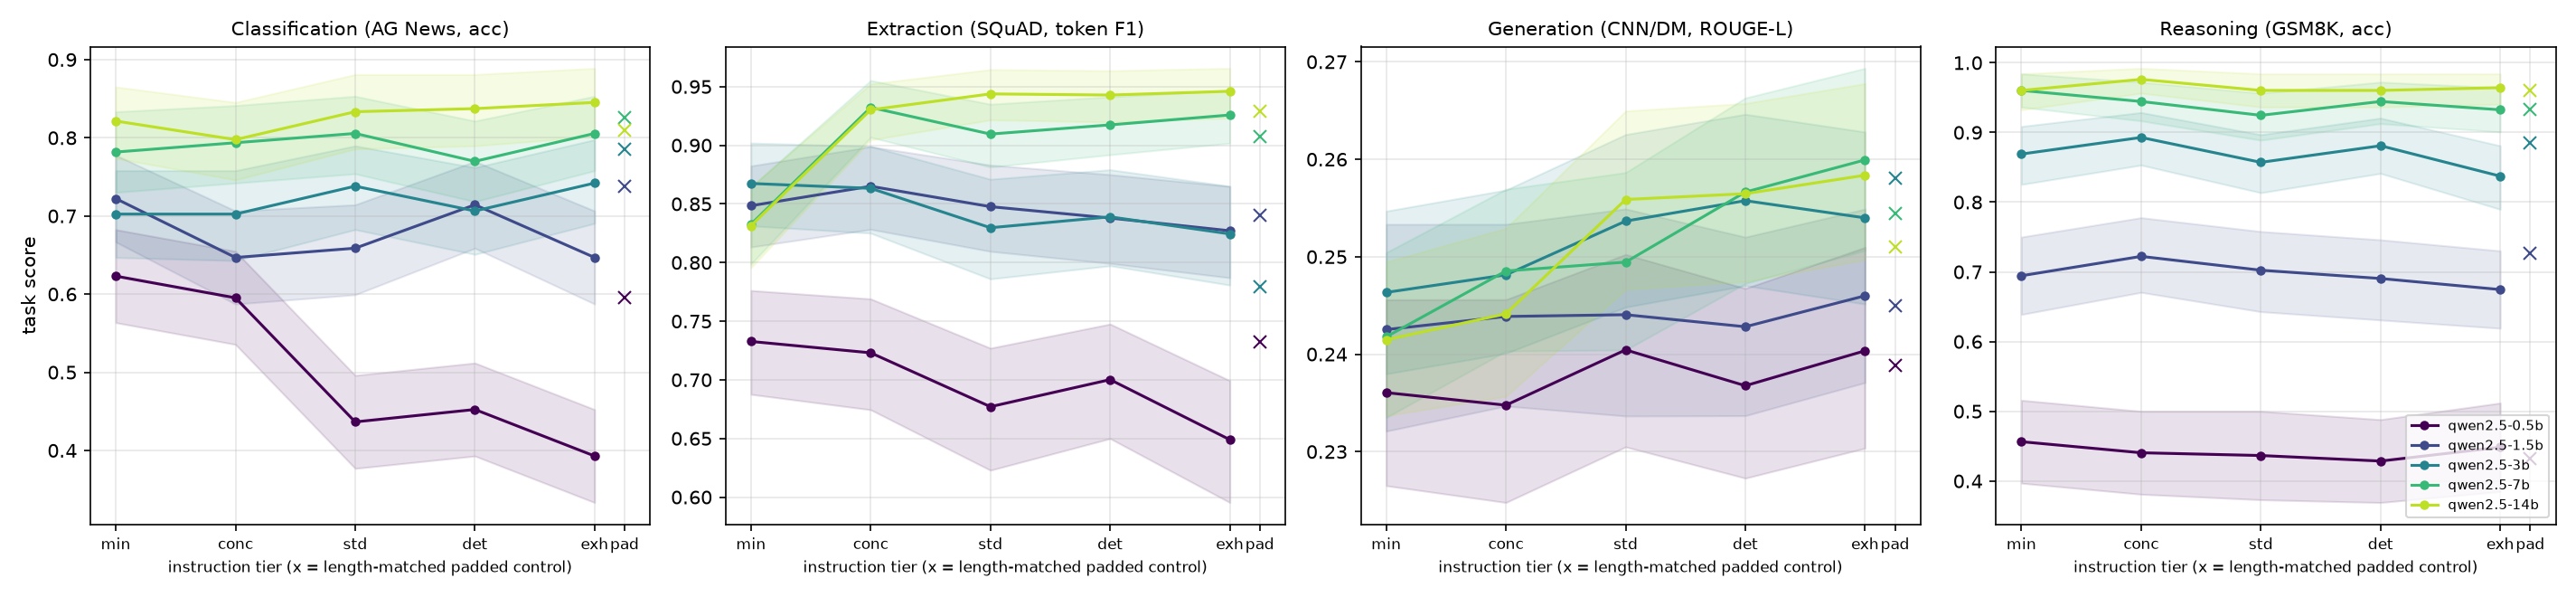
\includegraphics[width=\linewidth]{figures/score_by_tier.png}
\caption{Task score \versus instruction tier for five \qwen sizes. Shaded areas are 95\% bootstrap CIs; $\times$ marks the length-matched \padded control. For $\geq$3B models the curves are flat or slowly rising after \concise. The only steep decline is the 0.5B model on classification (and, more mildly, extraction), and the \padded control (same content as \standard, length of \exhaustive) sits near the \minimal level rather than the \exhaustive level.}
\label{fig:scores}
\end{figure}

\begin{table}[t]
\centering
\caption{Task score (\%) by instruction tier, $n=252$ items per cell. Classification and reasoning are accuracy, extraction is token F1, and generation is ROUGE-L F1. The best condition per row is in {\bf bold}. Binary-metric 95\% CIs are about $\pm$5--6 points; ROUGE-L CIs are about $\pm$1 point. For $\geq$3B models, \standard and \exhaustive are within 1.6 points on every task. Only the 0.5B model shows a large decline with length, and the \padded control does not reproduce it.}
\label{tab:main}
\small
\begin{tabular}{@{}llcccccc@{}}
\toprule
Task & Model & \minimal & \concise & \standard & \detailed & \exhaustive & \padded \\
\midrule
\multirow{5}{*}{\shortstack[l]{\textsc{Cls}\\(\agnews)}}
 & 0.5B & {\bf 62.3} & 59.5 & 43.7 & 45.2 & 39.3 & 59.5 \\
 & 1.5B & 72.2 & 64.7 & 65.9 & 71.4 & 64.7 & {\bf 73.8} \\
 & 3B   & 70.2 & 70.2 & 73.8 & 70.6 & 74.2 & {\bf 78.6} \\
 & 7B   & 78.2 & 79.4 & 80.6 & 77.0 & 80.6 & {\bf 82.5} \\
 & 14B  & 82.1 & 79.8 & 83.3 & 83.7 & {\bf 84.5} & 81.0 \\
\midrule
\multirow{5}{*}{\shortstack[l]{\textsc{Ext}\\(\squad)}}
 & 0.5B & {\bf 73.3} & 72.3 & 67.7 & 70.0 & 64.9 & 73.2 \\
 & 1.5B & 84.8 & {\bf 86.5} & 84.8 & 83.8 & 82.7 & 84.0 \\
 & 3B   & {\bf 86.7} & 86.3 & 83.0 & 83.9 & 82.4 & 77.9 \\
 & 7B   & 83.3 & {\bf 93.2} & 91.0 & 91.7 & 92.6 & 90.8 \\
 & 14B  & 83.1 & 93.0 & 94.4 & 94.3 & {\bf 94.6} & 92.9 \\
\midrule
\multirow{5}{*}{\shortstack[l]{\textsc{Gen}\\(\cnndm)}}
 & 0.5B & 23.6 & 23.5 & {\bf 24.0} & 23.7 & {\bf 24.0} & 23.9 \\
 & 1.5B & 24.3 & 24.4 & 24.4 & 24.3 & {\bf 24.6} & 24.5 \\
 & 3B   & 24.6 & 24.8 & 25.4 & 25.6 & 25.4 & {\bf 25.8} \\
 & 7B   & 24.2 & 24.9 & 24.9 & 25.7 & {\bf 26.0} & 25.4 \\
 & 14B  & 24.1 & 24.4 & 25.6 & 25.6 & {\bf 25.8} & 25.1 \\
\midrule
\multirow{5}{*}{\shortstack[l]{\textsc{Rsn}\\(\gsm)}}
 & 0.5B & {\bf 45.6} & 44.0 & 43.7 & 42.9 & 44.8 & 43.3 \\
 & 1.5B & 69.4 & 72.2 & 70.2 & 69.0 & 67.5 & {\bf 72.6} \\
 & 3B   & 86.9 & {\bf 89.3} & 85.7 & 88.1 & 83.7 & 88.5 \\
 & 7B   & {\bf 96.0} & 94.4 & 92.5 & 94.4 & 93.3 & 93.3 \\
 & 14B  & 96.0 & {\bf 97.6} & 96.0 & 96.0 & 96.4 & 96.0 \\
\bottomrule
\end{tabular}
\end{table}


\subsection{Task scores are flat across tiers for models of 3B and above}
\label{sec:res_scores}

\Figref{fig:scores} and \tabref{tab:main} show task scores for all conditions.
{\bf For 3B--14B models, the curves are flat after the first step.}
Classification accuracy for 7B stays between 77.0\% and 80.6\% across all five tiers, and 14B stays between 79.8\% and 84.5\%.
Reasoning accuracy for 14B ranges only from 96.0\% to 97.6\%.
Where we see a clear change, it comes from the shortest instruction.
For extraction, moving from \minimal to \concise raises 7B F1 from 83.3 to 93.2 and 14B F1 from 83.1 to 93.0.
The \minimal prompt makes models return spans that are too long: the 7B model's mean answer length is 5.0 words at \minimal and 3.1--3.3 words at every longer tier.
Once the instruction defines what a good span is, further detail neither helps nor hurts.

{\bf Generation improves slowly and does not plateau.}
ROUGE-L for $\geq$3B models rises from 24.1--24.6 at \minimal to 25.4--26.0 at \exhaustive.
The per-tier slope from \minimal to \detailed is $+0.34$ [0.10, 0.57] points for 3B, $+0.45$ [0.21, 0.69] for 7B, and $+0.57$ [0.32, 0.82] for 14B.
Every consecutive step is positive, but no single step is significant on its own.
The gain continues to \exhaustive rather than peaking at \detailed.
The 0.5B and 1.5B models show a slope of about zero.

{\bf The smallest model is the exception.}
For 0.5B, the \minimal tier is the best tier on three of four tasks.
Classification accuracy drops from 62.3\% at \minimal to 43.7\% at \standard and 39.3\% at \exhaustive, and extraction F1 drops from 73.3 to 64.9.

\subsection{The standard-to-exhaustive drop shrinks with model size, but 7B is not special}
\label{sec:res_drop}

\begin{table}[t]
\centering
\caption{Primary contrast: \standard $-$ \exhaustive, in points with 95\% bootstrap CIs. Positive values mean the \exhaustive tier hurts. Uncorrected permutation $p$-values are shown where $p<.1$. After Holm correction over these 20 tests, only 7B generation is significant ($p_{\text{holm}}=.02$), and there \exhaustive \emph{helps}. The 0.5B classification drop has $p_{\text{holm}}=.25$.}
\label{tab:drop}
\small
\begin{tabular}{@{}lcccc@{}}
\toprule
Model & \textsc{Cls} & \textsc{Ext} & \textsc{Gen} & \textsc{Rsn} \\
\midrule
0.5B & $+4.4$ {\scriptsize [1.2, 7.5]} $p{=}.013$ & $+2.8$ {\scriptsize [$-1.2$, 6.7]} & \phantom{$+$}$0.0$ {\scriptsize [$-0.7$, 0.7]} & $-1.2$ {\scriptsize [$-7.5$, 5.2]} \\
1.5B & $+1.2$ {\scriptsize [$-2.0$, 4.4]} & $+2.1$ {\scriptsize [$-0.7$, 4.9]} & $-0.2$ {\scriptsize [$-0.9$, 0.5]} & $+2.8$ {\scriptsize [$-2.8$, 8.3]} \\
3B   & $-0.4$ {\scriptsize [$-4.0$, 3.2]} & $+0.5$ {\scriptsize [$-2.5$, 3.5]} & \phantom{$+$}$0.0$ {\scriptsize [$-0.6$, 0.6]} & $+2.0$ {\scriptsize [$-2.0$, 6.3]} \\
7B   & \phantom{$+$}$0.0$ {\scriptsize [$-2.4$, 2.4]} & $-1.6$ {\scriptsize [$-3.5$, 0.0]} $p{=}.06$ & {\bf $-$1.0} {\scriptsize [$-1.7$, $-0.4$]} $p{=}.001$ & $-0.8$ {\scriptsize [$-4.4$, 2.8]} \\
14B  & $-1.2$ {\scriptsize [$-4.4$, 2.0]} & $-0.2$ {\scriptsize [$-1.3$, 0.8]} & $-0.2$ {\scriptsize [$-0.8$, 0.3]} & $-0.4$ {\scriptsize [$-2.4$, 1.6]} \\
\bottomrule
\end{tabular}
\end{table}


\begin{figure}[t]
\centering
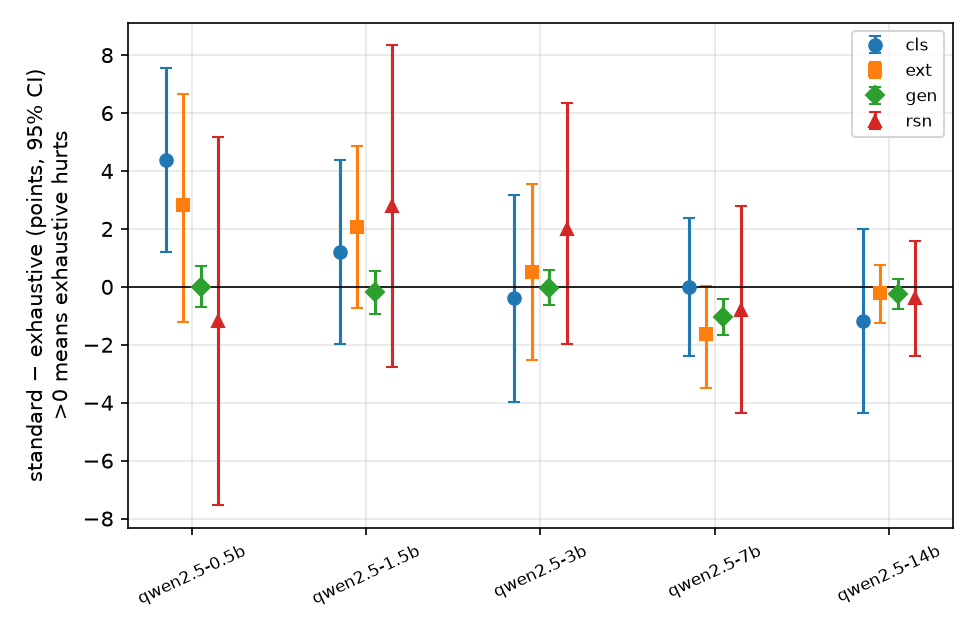
\includegraphics[width=0.6\linewidth]{figures/drop_by_model.png}
\caption{\standard $-$ \exhaustive difference per model and task, with 95\% bootstrap CIs. Values above zero mean the longer instruction hurts. Only the 0.5B classification interval lies fully above zero; for 7B and 14B all point estimates are at or below zero.}
\label{fig:drop}
\end{figure}

H1 predicts a 3--7 point drop from \standard to \exhaustive for classification and extraction.
\Tabref{tab:drop} and \figref{fig:drop} show that this drop does not appear for models of 1.5B and above.
For $\geq$1.5B, the drop is at most $+1.2$ points on classification and $+2.1$ on extraction, and no interval excludes zero in the predicted direction.
For 7B and 14B, all point estimates are zero or negative, so the longer instruction is, if anything, slightly better.
After Holm correction over the 20 primary tests, the only significant difference is 7B generation, where \exhaustive is 1.0 ROUGE-L point \emph{better} ($p_{\text{holm}}=.02$).
The 0.5B classification drop of 4.4 points is significant before correction ($p=.013$) but not after ($p_{\text{holm}}=.25$).

H4 predicts that 7B degrades more than larger models.
It does not: the 7B $-$ 14B difference-in-differences is $+1.2$ [$-3.2$, 5.6] for classification, $-1.4$ [$-3.4$, 0.5] for extraction, $-0.8$ for generation, and $-0.4$ for reasoning, all not significant.
A generalized form of H4 does hold.
Across the five sizes, the \standard$\to$\exhaustive drop decreases with log model size (Spearman $\rho=-0.9$, $p=.037$, for both classification and extraction).
With only five points this correlation is fragile, and the effect is concentrated below 2B parameters rather than spread across the range.

H3 predicts no change in reasoning beyond \concise.
Cochran's Q over \concise$\to$\exhaustive gives $p=.93$, .37, .056, .50, and .30 for the five sizes, so we find no significant differences.
However, we cannot establish equivalence within $\pm$3 points for most models, and 3B shows a 5.6-point dip from \concise to \exhaustive (90\% CI [$-9.5$, $-1.6$]).
The \exhaustive tier also changes \emph{how} models reason.
The 7B model follows the prescribed verification steps and produces outputs twice as long (437 \versus 214 tokens at \standard), with no change in accuracy.

\subsection{Format compliance saturates early}
\label{sec:res_compliance}

\begin{figure}[t]
\centering
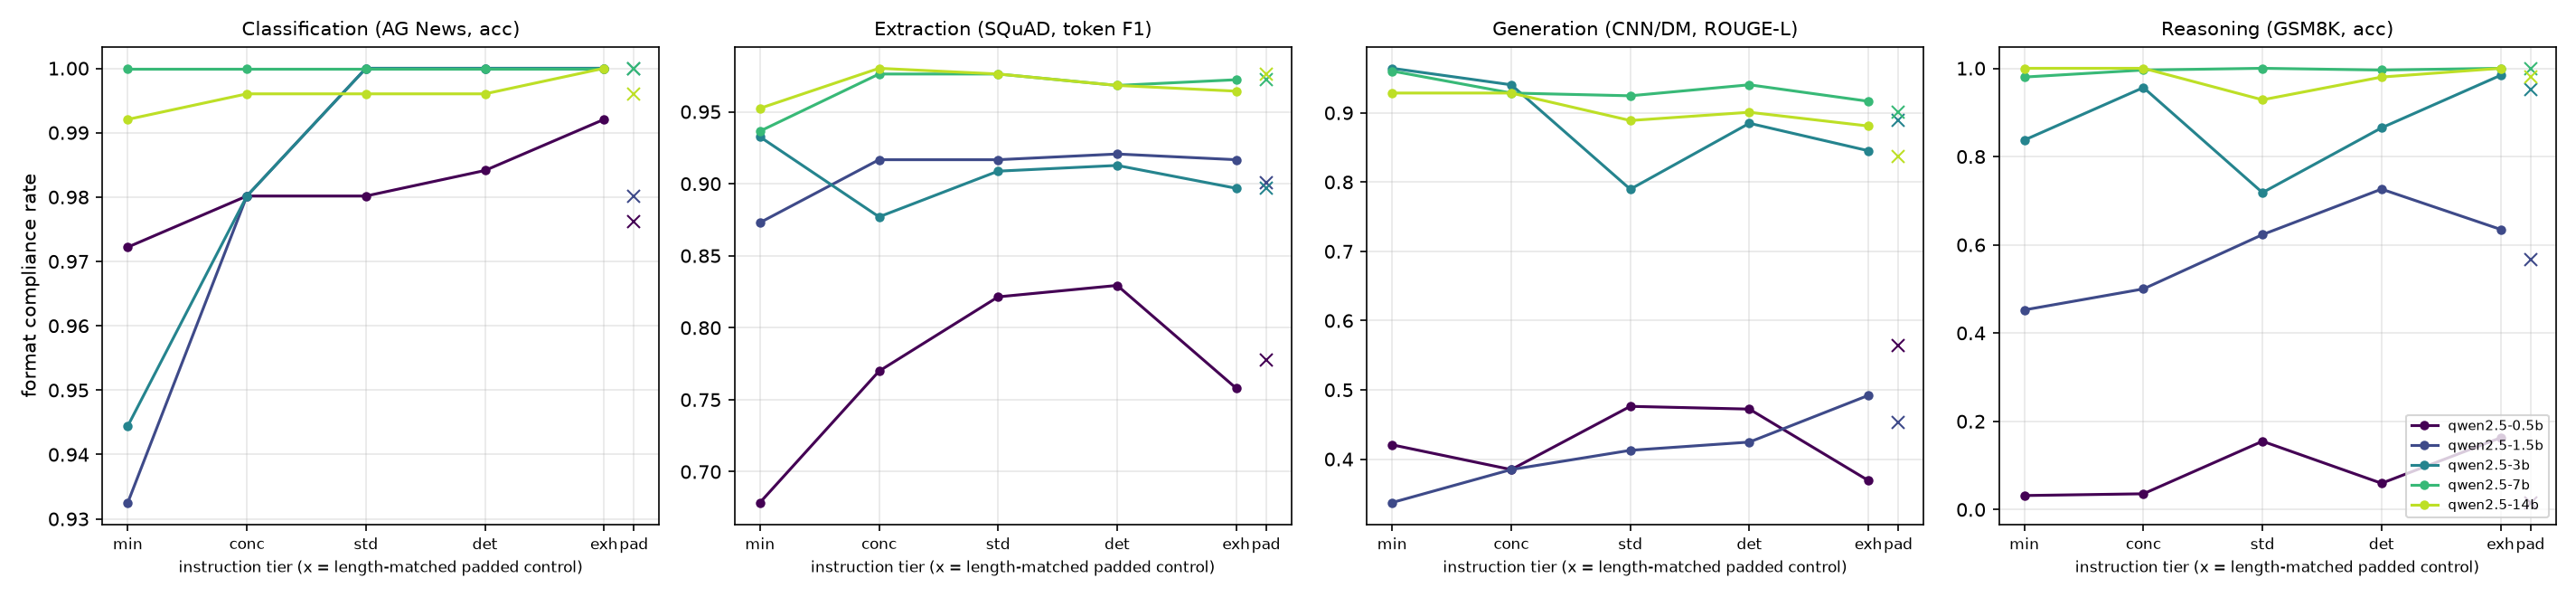
\includegraphics[width=\linewidth]{figures/compliance_by_tier.png}
\caption{Strict format-compliance rate \versus instruction tier (panel titles name the task; the y-axis is compliance, not task score). $\times$ marks the \padded control. Models of 7B and above reach 88--100\% compliance from \concise onward. The small models show no common peak, and for reasoning the \exhaustive tier, which ends by restating the format, is often the most compliant.}
\label{fig:compliance}
\end{figure}

H5 predicts that compliance peaks at \standard for every task.
\Figref{fig:compliance} shows that it does not.
\standard is the unique maximum in only 1 of 20 model$\times$task cells (0.5B generation), and is tied for the maximum in 5 more cells, all at or near 100\%.
The common pattern is a ceiling from \concise onward: $\geq$7B models comply 88--100\% of the time at every tier from \concise to \exhaustive.
For small models the peak tier is scattered.
Restating the format at the end of the prompt matters for reasoning: 3B compliance is 72\% at \standard and 98\% at \exhaustive.
Most reasoning violations are cosmetic, such as bold markdown (\texttt{**Final answer: 20**}) or LaTeX layouts.
The 0.5B and 1.5B models violate the generation constraint (2--4 sentences, $\leq$80 words) more than half the time at every tier.

\subsection{Length alone does not hurt: padding and placement controls}
\label{sec:res_padding}

\begin{table}[t]
\centering
\caption{Padding control. \padded has the content of \standard and the word count of \exhaustive. Differences are in points with 95\% bootstrap CIs; $p_{\text{holm}}$ is corrected over the 40 padding tests. Filler never significantly hurts after correction; for the small models it significantly \emph{helps} relative to \standard, while the content-rich \exhaustive tier is significantly worse than \padded.}
\label{tab:padding}
\resizebox{\textwidth}{!}{%
\begin{tabular}{@{}lccccc@{}}
\toprule
Model / task & \standard & \exhaustive & \padded & \padded $-$ \standard & \exhaustive $-$ \padded \\
\midrule
0.5B \textsc{Cls} & 43.7 & 39.3 & {\bf 59.5} & $+15.9$ {\scriptsize [11.1, 20.6]} \increase & $-20.2$ {\scriptsize [$-25.4$, $-15.1$]} \decrease \\
1.5B \textsc{Cls} & 65.9 & 64.7 & {\bf 73.8} & $+7.9$ {\scriptsize [4.4, 11.9]} \increase & $-9.1$ {\scriptsize [$-13.1$, $-5.2$]} \decrease \\
0.5B \textsc{Ext} & 67.7 & 64.9 & {\bf 73.2} & $+5.5$ {\scriptsize [0.9, 10.3]} & $-8.3$ {\scriptsize [$-12.9$, $-3.8$]} \decrease \\
\midrule
$\geq$3B, all tasks & \multicolumn{5}{c}{all differences within $\pm$5.1 points; none significant after correction} \\
\bottomrule
\end{tabular}%
}
\end{table}

H6 asks whether any harm from long instructions comes from token count or from content.
\Tabref{tab:padding} gives a clear answer: {\bf irrelevant filler of the same length does not reproduce the harm.}
For 0.5B classification, \padded reaches 59.5\%, 15.9 points above \standard and 20.2 points above \exhaustive ($p_{\text{holm}}=.008$ for both).
1.5B classification shows the same pattern ($+7.9$ and $-9.1$ points, $p_{\text{holm}}=.008$), and \exhaustive is 8.3 points below \padded for 0.5B extraction ($p_{\text{holm}}=.014$).
For $\geq$3B models, no padding difference survives correction.
The largest uncorrected effect is 3B extraction, where \padded is 5.1 points below \standard ($p=.005$ uncorrected), so filler is not entirely harmless; but across 40 tests it never significantly hurts after correction.
We therefore reject the pure token-dilution account in this length range.

\para{Instruction placement.}
Because \padded differs from \standard both in length and in what sits immediately before the input, we also move the instruction into the system message for 0.5B and 1.5B.
With system placement, 0.5B classification accuracy is 76.6, 71.8, 67.9, 71.8, and 64.3\% from \minimal to \exhaustive, compared with 62.3, 59.5, 43.7, 45.2, and 39.3\% in the user turn.
The sharp drop at \standard largely disappears, but a monotone decline of about 12 points from \minimal to \exhaustive remains.
Extraction shows the same pattern (78.7 to 71.5 F1).
For 1.5B, the curves are flat to slightly declining under both placements.

\para{Error analysis.}
The 0.5B classification drop is a label-collapse bias.
The model predicts ``Business'' for 152 of 252 items at \minimal, 199 at \standard, and 213 at \exhaustive, while the true count is 63.
This is not simple keyword frequency: the four label names are mentioned at similar rates in every tier (\eg 14, 11, 13, and 11 mentions in \exhaustive).
For $\geq$3B models, classification errors are dominated by Sci/Tech$\to$Business confusions (21--35 per condition for 7B), mostly technology-company business stories that \agnews labels inconsistently, and their count barely changes with tier.
Extraction errors shift from over-long spans at \minimal to a small residual of non-verbatim or wrong spans.
Reasoning errors for $\geq$3B models are almost entirely wrong numbers.

\begin{table}[t]
\centering
\caption{Verdicts for the pre-registered hypotheses.}
\label{tab:verdicts}
\small
\begin{tabular}{@{}p{0.36\linewidth}p{0.14\linewidth}p{0.44\linewidth}@{}}
\toprule
Hypothesis & Verdict & Key evidence \\
\midrule
H1: \textsc{Cls}/\textsc{Ext} peak at \standard, drop 3--7 pts at \exhaustive & Not supported & \standard$-$\exhaustive $\leq$ +1.2 (\textsc{Cls}) and $\leq$ +2.1 (\textsc{Ext}) for $\geq$1.5B, all n.s.; 0.5B peaks at \minimal. \\
H2: generation rises monotonically to \detailed & Partially & Positive slopes for $\geq$3B ($+0.34$ to $+0.57$ pts/tier); flat for $\leq$1.5B; gains continue to \exhaustive. \\
H3: reasoning flat beyond \concise & Largely & No significant differences (Cochran's Q); equivalence within $\pm$3 pts not established. \\
H4: 7B hurt more than larger models & Not supported & 7B$-$14B DiD n.s. on all tasks; drop shrinks with size ($\rho=-0.9$), mostly below 2B. \\
H5: compliance peaks at \standard & Not supported & Unique peak in 1/20 cells; ceiling from \concise for $\geq$7B. \\
H6: harm is token dilution & Refuted & Length-matched filler never significantly hurts; content-rich \exhaustive does (small models). \\
\bottomrule
\end{tabular}
\end{table}

\section{Discussion}
\label{sec:discussion}

{\bf Why does more detail not hurt 7B and 14B models?}
Our longest prompts are 1{,}000--1{,}700 tokens, far below the multi-thousand-token regimes where context-length degradation has been reported~\citep{liu2024lost,levy2024same}.
Our \exhaustive tiers are also consistent: they elaborate the task and never contradict it.
Under these conditions, extra rules are either redundant (classification, reasoning) or mildly useful (span boundaries in extraction, ``lead with the most newsworthy fact'' in summarization).
The main lever is the first step from \minimal to a short, specific instruction; beyond that, length is close to neutral.
The cost of a long instruction shows up elsewhere: the 7B model doubles its reasoning length when told to verify its work, which raises latency and cost without changing accuracy.

{\bf What goes wrong in tiny models?}
The 0.5B model's failure is a shift in its default label, not a loss of the format.
Two observations point to the text immediately before the input as the cause.
First, \padded has exactly the same task content as \standard but recovers most of the accuracy; the only difference is that the article follows neutral prose instead of a rule list ending in ``Output exactly one of \ldots (World, Sports, Business, Sci/Tech).''
Second, moving the instruction to the system message removes most of the drop at \standard.
For a 0.5B model, rules about companies, markets, and technology placed right before the article seem to prime the ``Business'' label, much like the recency bias reported for few-shot demonstrations~\citep{zhao2021calibrate}.
This is an interference effect of content and position, not a dilution effect of length.
A residual decline of about 12 points under system placement shows that small models are also harmed by detailed rule content itself.

{\bf Practical implications.}
Our results support four simple rules.
(1) Always include a short, task-specific definition; \minimal prompts leave about 10 F1 points on the table for extraction.
(2) For $\geq$3B instruction-tuned models, extra detail is cheap insurance with no measurable accuracy cost, but it can lengthen outputs.
(3) Restate the output format at the end of a long prompt; this made \exhaustive the most compliant tier for reasoning.
(4) For sub-2B models, prefer minimal instructions, or put them in the system message.

\subsection{Limitations}
\label{sec:limitations}

\para{One model family.}
All five models are \qwen. The planned Llama-3.1-8B and \qwen-32B runs could not be completed because the shared GPUs were occupied, so conclusions about ``larger models'' rest on 14B alone and cross-family generality is untested.

\para{One wording per tier.}
Within a tier, wording and length are confounded.
The nested design and the padding control reduce this problem but do not remove it.
A different \exhaustive prompt, for example one with conflicting or over-specific rules, could well hurt; ours were written to be realistic and consistent.

\para{Imperfect padding control.}
\padded is word-matched, which gives 7--12\% fewer tokens than \exhaustive.
It also changes what precedes the input, so the \padded\versus\standard comparison mixes length with recency.

\para{Statistical power.}
With $n=252$ per cell, binary-metric CIs are about $\pm$5--6 points, so the power to detect a 3-point effect in a single cell is low.
The size correlation uses only five points.

\para{Metrics and decoding.}
ROUGE-L is a coarse proxy for summary quality, and we did not run human or LLM-judge evaluation.
\agnews labels are noisy, which caps accuracy at roughly 85--90\%.
Compliance definitions are strict and chosen by us.
We use greedy decoding with a single seed and capture variability only through item resampling.
All four datasets are public and likely seen in pre-training, which affects absolute levels more than within-model comparisons across tiers.

\para{Broader impact.}
This work aims to help practitioners write better prompts and does not introduce new capabilities.
A risk is over-generalization: our finding that detail is harmless for $\geq$3B models comes from one family at moderate prompt lengths and should not be read as a guarantee for every model or for very long agent prompts.

\section{Conclusion}
\label{sec:conclusion}

We asked whether longer, more detailed task instructions help or hurt instruction-tuned language models.
Using a nested five-tier instruction ladder over four task types and five \qwen sizes, with a length-matched padding control, we find that more detail mostly does not hurt.
For 3B--14B models, task performance from \standard to \exhaustive is flat for classification and reasoning and rises slightly for generation, and the predicted 3--7 point penalty does not appear.
Harm from long instructions is a small-model effect (0.5B and partly 1.5B), and it is driven by instruction content and its position before the input, not by token count.
The key takeaway is simple: give the model a short, specific task definition, and for capable models feel free to add detail beyond that.

Future work should test other model families (Llama, Gemma) and larger or API-only models, write several paraphrases per tier to separate wording from length, build ``adversarial-realistic'' long prompts with conflicting or excessive rules, extend the ladder to 5k--20k-token agent system prompts, evaluate generation with human or LLM judges, and use padding controls that are token-matched at both the start and the end of the instruction to separate recency from length.


\bibliography{references}

\appendix
\section{Experimental Details}
\label{app:details}

\para{Example tiers.}
The classification \minimal tier is: ``Classify the news article into one of these categories: World, Sports, Business, Sci/Tech. Respond with only the category name.''
The \concise tier adds one-line definitions of each category (\eg ``Business: companies, markets, the economy, and finance'').
The \standard tier adds five numbered guidelines, such as ``Articles about a technology company's earnings, stock price, mergers, or lawsuits are usually Business; articles about its products, software, research, or security problems are usually Sci/Tech,'' and ends with ``Output exactly one of the four category names, spelled exactly as given (World, Sports, Business, Sci/Tech), with no explanation, punctuation, or extra words.''
The \detailed tier adds guidance for difficult domains (health, energy, space, telecom, courts) and a tie-breaking rule.
The \exhaustive tier adds the purpose of the task, extended definitions, a step-by-step procedure, common mistakes, a restated format, and a final reminder.
The \padded filler begins: ``Background information about this project (not needed for the task): The documentation program that produced these materials began several years ago as a small internal initiative within the operations group\ldots''

\para{Compute.}
Runs used one slice (5--42\,GB) of a shared NVIDIA RTX A6000 (48\,GB).
A full model run of 6{,}048 prompts took about 2 minutes for 0.5B and 1.5B, 11 minutes for 7B, and 80 minutes for 14B (slowed by memory contention).

\para{Software.}
Python 3.12, vLLM 0.32.0, PyTorch 2.13, pandas 3.0.6, NumPy 2.3.5, SciPy 1.18.1, and rouge-score 0.1.2.
Data sampling, vLLM, and bootstrap all use seed 42.
Raw generations for every prompt are stored with the code.

\para{Statistical tests.}
Bootstrap CIs use 5{,}000 item resamples.
Paired differences use a two-sided sign-flip permutation test.
Holm correction is applied within the 20 primary \standard\versus\exhaustive tests and within the 40 padding tests.
We also applied Holm correction across all 320 score and compliance comparisons. This is very conservative: 32 comparisons remain significant ($p_{\text{holm}}=.03$ each, the floor set by the number of permutations). They include the 0.5B classification drops from \minimal and \concise to \standard (18.7 and 15.9 points), the 0.5B and 1.5B classification gains of \padded over \standard, the \minimal$\to$\concise extraction gains for 7B and 14B (10.0 and 9.9 F1), and the 26.6-point reasoning-compliance gain of \exhaustive over \standard for 3B. No \standard\versus\exhaustive \emph{score} difference survives this correction.


\end{document}
